\documentclass[11pt]{article}
\usepackage[margin=0.82in]{geometry}
\usepackage[T1]{fontenc}
\usepackage{lmodern}
\usepackage{microtype}
\usepackage{amsmath}
\usepackage{booktabs,longtable,tabularx,array}
\usepackage{enumitem}
\usepackage{xcolor}
\usepackage{hyperref}
\usepackage{xurl}
\usepackage{fancyhdr}
\usepackage{tikz}
\usepackage{graphicx}
\usepackage{float}
\usepackage{placeins}
\usepackage{makecell}
\usepackage[numbers,sort&compress]{natbib}
\usepackage{tcolorbox}
\tcbuselibrary{breakable}
\newcommand{\plainbox}[2]{\begin{tcolorbox}[colback=#1!6,colframe=#1!55,boxrule=0.6pt,arc=2pt,left=6pt,right=6pt,top=4pt,bottom=4pt]#2\end{tcolorbox}}

\graphicspath{{figures/}}
\usetikzlibrary{arrows.meta,positioning}
\hypersetup{hidelinks,pdfauthor={Rajeev Yadav, Ph.D.},pdftitle={FinCompass User Guide}}
\setlength{\parindent}{1em}
\setlength{\parskip}{0.3em}
\setlength{\emergencystretch}{2em}
\newcommand{\FC}{\textsc{FinCompass}}
\newcommand{\logit}{\operatorname{logit}}
\pagestyle{fancy}
\fancyhf{}
\fancyhead[L]{\small FinCompass User Guide}
\fancyhead[R]{\small Rajeev Yadav, Ph.D.}
\fancyfoot[C]{\thepage}
\title{\textbf{FinCompass User Guide}}
\author{Rajeev Yadav, Ph.D.}
\date{August 2026}
\begin{document}
\maketitle
\begin{center}
\large Research, forecasting, model governance and quantitative analytics in one local workbench
\end{center}
\vspace{1em}
\noindent\textbf{Purpose.} This guide explains how to use \FC\ from first ticker entry through Forecast, Live, model maintenance and Research Details. The early sections focus on what to do and what the results mean. Later sections explain the mathematics, validation, data controls and model architecture in sufficient depth to audit the system.

\tableofcontents
\newpage

\section{What FinCompass is}
\FC\ is a local-first financial research workbench. It combines four kinds of analysis that are intentionally kept separate:
\begin{enumerate}[itemsep=0.2em]
\item an evidence score that summarizes currently observed company and market information;
\item a probabilistic Forecast for a precisely defined future event;
\item a Live workspace that tracks the frozen Forecast and may apply a separately governed adaptive adjustment when enough evidence has matured;
\item deterministic quantitative analytics such as performance, risk, ratios, DCF, bond mathematics, options, portfolio measures, factors and technical indicators.
\end{enumerate}

These outputs answer different questions. A high evidence score is not automatically a high probability of future outperformance. A DCF value is not a Forecast probability. A Sharpe ratio is a description of historical return and volatility, not a prediction.

\section{The normal workflow}
For a supported security, the intended user journey is short:
\begin{center}
\textbf{Enter ticker $\rightarrow$ FinCompass identifies the market $\rightarrow$ obtains or checks local data $\rightarrow$ selects the strongest applicable pooled model $\rightarrow$ Forecast $\rightarrow$ Start Live.}
\end{center}

\begin{figure}[H]
\centering
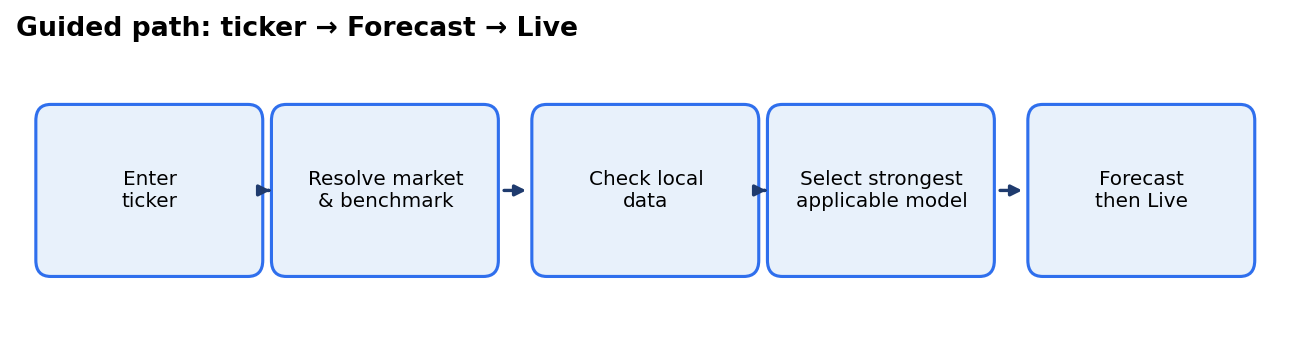
\includegraphics[width=0.98\textwidth]{guided_workflow.png}
\caption{The Guided path is a short sequence. Model IDs, hashes and locked-test metrics stay in Research Details.}
\end{figure}

\plainbox{blue}{\textbf{At a glance.} Type a ticker. FinCompass classifies the market, checks local data, picks the strongest applicable family model, and returns one probability. You do not train a new model for every name.}

You should not need to train a separate model for every new ticker. Pooled model families are designed to cover defined market domains. For example, a US common-stock family model may be applicable to a newly entered US common stock even if that ticker was not one of the securities used to fit the model.

If local data are missing, \FC\ should ask for an update and continue. If the family model is old, the software may recommend model maintenance, but an existing hard-valid applicable Forecast should remain available unless a documented hard-expiry rule is triggered.

\section{First use: entering a ticker}
Enter a ticker in the Forecast workspace. The software performs several steps internally:
\begin{enumerate}[itemsep=0.2em]
\item resolves the symbol and security identity;
\item classifies the asset class and market region;
\item chooses a benchmark policy;
\item checks whether local price history is sufficient;
\item searches the model registry for the strongest applicable model at the requested horizon;
\item checks scientific applicability, not merely whether the code can calculate features;
\item produces the Forecast when the required conditions are satisfied.
\end{enumerate}

The user interface should present these as simple readiness statements, not engineering internals. Model IDs, dataset hashes, locked-test thresholds and feature contracts belong in Research Details.

\section{Choosing a forecast period}
The forecast period determines the event being estimated. A six-month forecast and a twelve-month forecast are not interchangeable.

Suppose the displayed event is:
\begin{quote}
Probability that the security outperforms the S\&P 500 over the next 12 months.
\end{quote}
A value of 58\% means the model estimates a 0.58 probability of that exact event under its declared data and applicability contract. It does not mean:
\begin{itemize}[itemsep=0.15em]
\item the security will rise 58\%;
\item the model is 58\% accurate;
\item the security has a 58\% chance of making money on every path;
\item the expected return is 58\%;
\item the result is a recommendation.
\end{itemize}

\section{Understanding the benchmark}
Many \FC\ Forecasts are relative to a benchmark. If the benchmark is the S\&P 500, the event compares the security's future return with the S\&P 500 over the same horizon.

A security can decline in absolute terms and still outperform its benchmark. Conversely, it can rise and still underperform a stronger market. Always read the benchmark line before interpreting the probability.

\section{Reading the Forecast card}
\begin{figure}[H]
\centering
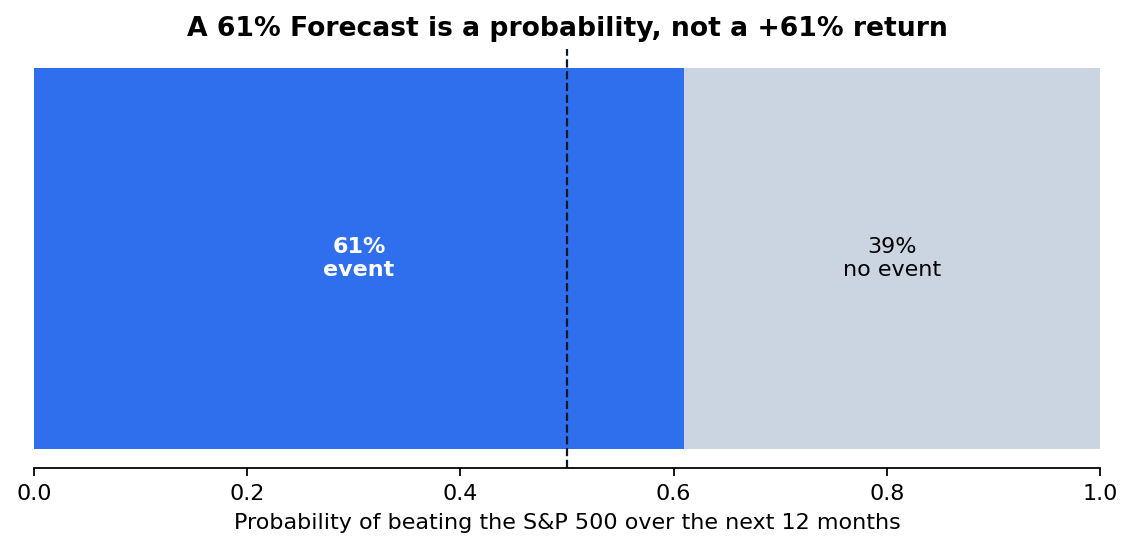
\includegraphics[width=0.82\textwidth]{probability_meaning.png}
\caption{A 61\% Forecast is the estimated probability of a named event. It is not a target return of $+61\%$.}
\end{figure}

A Forecast card should answer five questions immediately:
\begin{enumerate}[itemsep=0.2em]
\item \textbf{What is the probability?}
\item \textbf{What event is being forecast?}
\item \textbf{What is the horizon?}
\item \textbf{What benchmark is used?}
\item \textbf{How strong is the supporting evidence?}
\end{enumerate}

A typical card might read:
\begin{quote}
\textbf{54\%}\par
Estimated probability of outperforming the S\&P 500 over the next year.\par
\textbf{Evidence: Limited}
\end{quote}

The evidence label matters. It tells you whether the probability comes from a hard-valid Bayesian baseline or from a model that has passed stronger out-of-sample validation.

\section{Evidence labels}
\subsection{Limited evidence}
A Limited-evidence Forecast comes from a Bayesian baseline that passed hard validity checks but did not establish the stronger predictive skill required for the validated-research tier.

This means the model is usable as a probability reference but should be interpreted cautiously. It is not being presented as demonstrated alpha.

\subsection{Research validated}
A research-validated model passed the configured locked-test statistical and stability gates on its declared historical research corpus. This is stronger evidence than a baseline, but the result remains limited to the data, market, horizon and applicability domain recorded in the model manifest.

\subsection{Market validated}
This is the strongest model tier. In addition to the statistical gate, it requires stronger historical-universe and point-in-time controls such as survivorship handling, delistings and corporate-action treatment.

\section{Why a weak model can still produce a probability}
A model can be mathematically valid without showing meaningful incremental predictive skill. For example, it may converge, remain leakage-free, use a proper chronological split and produce reasonably calibrated probabilities, yet perform similarly to the historical event rate.

The correct conclusion is not necessarily ``the software failed.'' It is that the probability has limited demonstrated predictive evidence. \FC\ separates these two judgments so the stronger validation thresholds do not need to be weakened simply to make the product usable.

\section{Start Live}
After a Forecast is available, choose \textbf{Start Live}. The same button can lead to two scientifically different modes, selected automatically by the software.

\subsection{Tracking-only Live}
When the Forecast comes from a Limited-evidence Bayesian baseline, Live tracks the frozen probability and freshness state. It does not activate adaptive learning and does not apply a live residual. The current forecast therefore remains equal to the original forecast unless a different model is explicitly selected later.

This mode is still useful. It gives one place to monitor the Forecast, data recency and model status without overstating the evidence.

\subsection{Adaptive-eligible Live}
A research-validated or market-validated model may be eligible to serve as the anchor for the adaptive Live layer. Even then, the adaptive adjustment is not automatically applied. The Live gate must accumulate enough matured outcomes, enough distinct dates, enough elapsed time, acceptable probability losses, acceptable calibration and no active drift warning.

Until those conditions are met, the frozen Forecast remains in control.

\section{How to read Live}
The most important Live values are:
\begin{description}[style=nextline]
\item[Original forecast] The frozen anchor probability when Live was started.
\item[Current forecast] The probability currently being applied. It may equal the original forecast when the adaptive layer is inactive.
\item[Candidate forecast] A provisional adaptive estimate calculated from fresh context. It is not necessarily applied.
\item[Evidence status] Whether the adaptive layer is warming, active or degraded.
\end{description}

A healthy display might say:
\begin{quote}
Current forecast: 61\%\par
Original forecast: 62\%\par
New information suggests a small decrease. Live adjustment is not being applied yet because FinCompass is still collecting enough completed outcomes.
\end{quote}

That wording is more meaningful than exposing raw gate names or model-state codes.

\section{Data updates}
\FC\ keeps a durable local research corpus. Updating does not require downloading the entire history each time.

A normal update:
\begin{enumerate}[itemsep=0.2em]
\item starts shortly before the most recent retained date;
\item downloads a short overlap and the missing tail;
\item compares overlapping values;
\item records provider revisions;
\item appends genuinely new observations;
\item preserves raw source frames and hashes where configured.
\end{enumerate}

If the provider changes the price basis, such as raw versus adjusted history, \FC\ should rebuild the affected symbol instead of appending incompatible prices.

\section{Three kinds of freshness}
\begin{figure}[H]
\centering
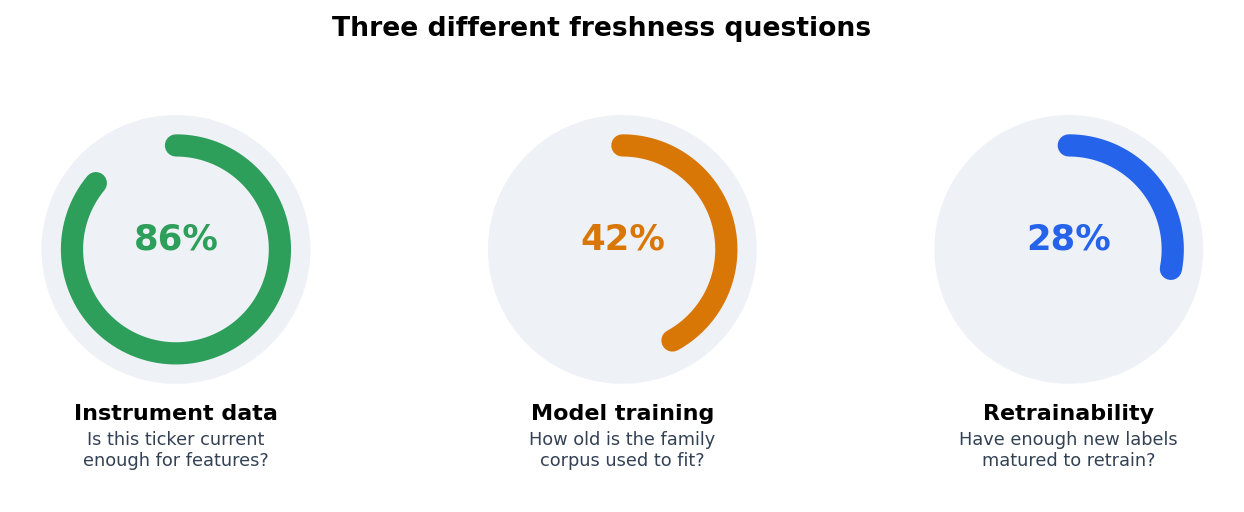
\includegraphics[width=0.98\textwidth]{freshness_clocks.png}
\caption{Instrument freshness, model-training freshness and retrainability answer three different questions. A current ticker price does not make a 2022 family model ``stale'' by itself.}
\end{figure}

The term ``freshness'' is easy to misuse. \FC\ should distinguish three separate concepts.

\subsection{Instrument-data freshness}
Are the ticker and benchmark histories current enough to build today's features?

\subsection{Model-training freshness}
How old was the family training corpus when the model was fitted?

\subsection{Retrainability}
Have enough new family observations and matured labels accumulated to justify or support a retrain?

A new ticker having data through today does not itself make a pooled family model stale. The model was trained on a family corpus, not on that newly entered ticker alone.

\section{Model maintenance}
Model maintenance is separate from obtaining a Forecast. If an applicable hard-valid model already exists, an update may be recommended while the current Forecast remains available.

When an update is launched, \FC\ should:
\begin{enumerate}[itemsep=0.2em]
\item keep the current model intact;
\item rebuild the training dataset from the accumulated local corpus;
\item include only matured forward outcomes;
\item train a new immutable candidate;
\item evaluate the candidate;
\item compare the newer model with the current model;
\item require an explicit replacement action for a stronger active model.
\end{enumerate}

If the candidate is not ready, fails computationally, or does not earn the intended evidence tier, the current Forecast should remain available.

\section{Why labels must mature}
Assume a Forecast horizon of one year. An observation made today cannot have a one-year outcome tomorrow. The software may use today's information to create a new Forecast, but that observation cannot become a supervised training label until the one-year endpoint actually occurs.

This rule prevents a major source of leakage. It also explains why adaptive Live learning can take time: each pending observation must wait for its original horizon to mature.

\section{The evidence workspace}
The evidence engine summarizes current information across five pillars:
\begin{itemize}[itemsep=0.15em]
\item Quality;
\item Financial Durability;
\item Safety;
\item Valuation;
\item Cycle.
\end{itemize}
Each pillar can include uncertainty and evidence coverage. Missing data should move the result toward neutral and widen uncertainty rather than being silently replaced by optimistic assumptions.

The evidence score is not a forward return probability. It is a structured research summary.

\section{Performance analytics}
\FC\ includes deterministic historical-performance measures.

\subsection{Annualized return}
For periodic returns $r_t$ and $m$ periods per year,
\begin{equation}
R_{ann}=\left(\prod_{t=1}^{T}(1+r_t)\right)^{m/T}-1.
\end{equation}
Annualization makes histories of different lengths easier to compare, but it does not imply the same return will continue.

\subsection{Volatility}
Annualized volatility is approximately
\begin{equation}
\sigma_{ann}=s_r\sqrt{m}.
\end{equation}
It summarizes dispersion of historical returns, not direction.

\subsection{Sharpe ratio}
The Sharpe ratio compares average excess return with total volatility. A higher historical Sharpe is not a guarantee of a better future outcome.

\subsection{Sortino ratio}
Sortino focuses on downside deviation rather than all volatility. It can be useful when upside and downside variability should not be treated symmetrically.

\subsection{Maximum drawdown}
Maximum drawdown is the largest peak-to-trough decline in the historical wealth path. It is a historical observation, not a worst-case bound.

\subsection{Beta and tracking error}
Beta describes historical sensitivity to a benchmark. Tracking error describes dispersion of active returns relative to the benchmark. Neither is itself a forecast.

\section{Risk analytics}
\subsection{Value at Risk}
VaR estimates a loss threshold under a stated model and confidence level. A 95\% one-day VaR is not the maximum possible one-day loss. Losses can exceed VaR.

\subsection{Expected shortfall}
Expected shortfall summarizes average loss beyond a VaR threshold under the historical or assumed distribution. It provides tail information that VaR alone does not.

\subsection{EWMA volatility}
Exponentially weighted volatility gives more weight to recent observations, allowing measured volatility to respond faster to changing market conditions.

\section{Technical analytics}
Technical calculations include moving averages, exponential moving averages, RSI, MACD, Bollinger Bands and ATR.

These can help describe trend, momentum and volatility. They do not automatically become Forecast features. An indicator must be separately admitted through the feature-governance process before it can influence the forecasting model.

\section{Financial statements and normalization}
Data providers use different field names and conventions. \FC\ converts provider-specific vocabulary into canonical income-statement, balance-sheet and cash-flow fields.

Every normalized value should carry enough context to identify whether it was reported directly, mapped from a provider alias, derived from other fields, unavailable or not applicable. Missing values remain missing. They are not silently converted to zero.

This matters because a missing inventory balance is not the same thing as zero inventory, and missing debt is not the same thing as no debt.

\section{Financial ratios}
Ratios are grouped into several families.

\subsection{Profitability}
Examples include gross margin, operating margin, net margin, return on assets and return on equity. Ratios with negative or structurally invalid denominators require careful interpretation.

\subsection{Liquidity}
Current ratio and quick ratio compare near-term resources with near-term obligations. Sector context matters: a bank and a manufacturer should not be interpreted using identical balance-sheet intuition.

\subsection{Leverage}
Debt-to-equity, debt-to-assets and interest-coverage measures describe capital structure and debt burden. Negative equity can make some common leverage ratios economically difficult to interpret; the software should not hide that problem by returning a convenient finite value.

\subsection{Efficiency}
Asset turnover, inventory turnover and receivables measures describe how efficiently resources are used. Period-average balance-sheet denominators are often preferable to a single ending balance when appropriate data are available.

\section{Discounted cash flow valuation}
DCF estimates present value under explicit assumptions. The unlevered free-cash-flow identity is
\begin{equation}
FCFF=EBIT(1-T)+D\&A-CapEx-\Delta NWC.
\end{equation}
Projected FCFF values are discounted at WACC. Terminal value may use perpetual growth or an exit multiple.

The output is only as reliable as the assumptions. A useful DCF workflow therefore emphasizes sensitivity analysis:
\begin{itemize}[itemsep=0.15em]
\item revenue growth;
\item operating margin;
\item tax rate;
\item reinvestment;
\item WACC;
\item terminal growth or exit multiple;
\item net debt and diluted shares.
\end{itemize}

Do not treat one DCF number as truth. Compare scenarios and inspect which assumptions dominate the result.

\section{Fixed-income analytics}
The fixed-income module calculates bond price, current yield, yield to maturity, Macaulay duration, modified duration, convexity and DV01 from explicit terms.

\subsection{Bond price}
For face value $F$, coupon $C$, yield $y$, frequency $m$ and $n$ remaining periods,
\begin{equation}
P=\sum_{k=1}^{n}\frac{C/m}{(1+y/m)^k}+\frac{F}{(1+y/m)^n}.
\end{equation}

\subsection{Duration}
Macaulay duration is a weighted average time to cash flow. Modified duration approximates percentage price sensitivity to a small yield change. Convexity improves the approximation for larger changes.

These are interest-rate sensitivity measures, not guaranteed future price changes.

\section{Options analytics}
European Black-Scholes-Merton calculations include theoretical call/put value and major Greeks.

\begin{description}[style=nextline]
\item[Delta] First-order sensitivity to the underlying price.
\item[Gamma] Change in Delta as the underlying changes.
\item[Vega] Sensitivity to volatility.
\item[Theta] Sensitivity to passage of time.
\item[Rho] Sensitivity to interest rates.
\end{description}

Actual option prices can differ because of volatility surfaces, liquidity, discrete dividends, early exercise and market microstructure. The calculation is a model result under stated assumptions.

\section{Portfolio analytics}
Portfolio analytics combine explicit holding weights with historical returns or a covariance matrix.

For weight vector $w$ and covariance matrix $\Sigma$,
\begin{equation}
\sigma_p^2=w^\top\Sigma w.
\end{equation}
Euler risk contributions can decompose portfolio volatility into holding-level contributions.

A portfolio probability should not be created by simply averaging the Forecast probabilities of its holdings. The joint distribution and dependence structure matter.

\section{Factor and regression analytics}
OLS factor models estimate descriptive exposures. A single-factor model may be written
\begin{equation}
r_i-r_f=\alpha+\beta(r_m-r_f)+\epsilon.
\end{equation}
A multi-factor model extends the right-hand side with additional factor returns.

The output includes coefficients, standard errors, t-statistics and fit measures. A statistically significant loading does not mean a factor tilt will generate future returns. In-sample exposure is not a forecast.

\section{The Bayesian reference model}
The standard Forecast baseline uses regularized Bayesian logistic regression. For feature vector $x$,
\begin{equation}
P(Y=1\mid x)=\frac{1}{1+\exp[-(\beta_0+x^\top\beta)]}.
\end{equation}
Shrinkage priors pull coefficients toward zero when the data do not strongly support large effects. This reduces instability and makes the model a useful reference against which more complex models can be judged.

The implementation approximates posterior coefficient uncertainty around the fitted mode and propagates that uncertainty into a probability range.

\section{Calibration in practical terms}
If a system repeatedly assigns 60\% probability to comparable events, a well-calibrated system should see those events occur approximately 60\% of the time over a sufficiently large and stable sample.

Calibration is therefore different from ranking. A model can be good at ranking companies from stronger to weaker while giving overconfident probabilities. Another model can have modest ranking power but reasonably calibrated probabilities.

\FC\ evaluates probability quality using proper scores and calibration diagnostics rather than relying on AUC alone.

\section{Brier score and log loss}
For one binary outcome $y$ and probability $p$,
\begin{equation}
BS=(p-y)^2.
\end{equation}
Lower is better. Brier skill compares the model with a reference forecast such as the historical event rate.

Log loss is
\begin{equation}
LL=-[y\log p+(1-y)\log(1-p)].
\end{equation}
It penalizes highly confident wrong predictions more strongly.

These metrics are appropriate because the model is trying to produce probabilities, not merely class labels.

\section{ROC AUC}
ROC AUC measures ranking. AUC of 0.5 corresponds to random ranking in a balanced conceptual sense; values above 0.5 indicate better ordering of positive and negative outcomes.

AUC is useful but insufficient. A high-AUC model can be badly calibrated, and a probability product must care about both ranking and probability accuracy.

\section{Why the test is locked}
The locked test is meant to represent data not used in model design. If you repeatedly change features after seeing the locked-test result, the test is no longer locked. It has become another development set.

\FC\ therefore separates:
\begin{itemize}[itemsep=0.15em]
\item training;
\item validation/calibration;
\item ensemble-weight selection where applicable;
\item final calibration;
\item locked testing.
\end{itemize}

Chronological purging and embargo rules further reduce leakage from overlapping forward horizons.

\section{Regime-aware Bayesian research model}
Markets can behave differently during stress, neutral and risk-on environments. The regime-aware model introduces a hidden market state estimated from benchmark-only, backward-looking features.

A three-state Gaussian hidden Markov model estimates filtered probabilities for the states. These probabilities are appended to the Bayesian reference features. Later test observations are processed forward so future data cannot rewrite earlier state assignments.

The regime model is not assumed to be better. It must demonstrate incremental value. On the current reference corpus, some horizons improved selected metrics while others worsened. The model therefore remains a research alternative rather than the default.

\section{Enhanced model}
The enhanced model combines Bayesian logistic regression with nonlinear learners such as histogram gradient boosting and random forest. Separate chronological stages are used for component calibration, ensemble weighting and final calibration.

The important principle is not the exact list of algorithms. The principle is that complexity must improve on the simpler reference under protected out-of-sample evaluation. If it does not, the simpler model should remain preferred.

\section{Current reference evidence}
The current bundled research evidence uses a small historical US-equity sample and the S\&P 500. It is useful for demonstrating software behavior and the validation framework but is not a survivorship-complete market dataset.

\begin{table}[ht]
\centering
\caption{Bayesian reference results on the declared locked tests.}
\begin{tabular}{rrrrr}
\toprule
Horizon & Test $n$ & AUC & Brier skill & ECE\\
\midrule
6 months & 539 & 0.419 & -0.023 & 0.056\\
12 months & 532 & 0.480 & -0.012 & 0.035\\
24 months & 518 & 0.415 & -0.004 & 0.064\\
36 months & 497 & 0.303 & -0.108 & 0.199\\
\bottomrule
\end{tabular}
\end{table}

These models are retained as Limited-evidence baselines. They are not promoted to stronger tiers merely because the software can fit them.

The stronger twelve-month enhanced model recorded approximately AUC 0.576, Brier skill 0.036, log-loss skill 0.027 and ECE 0.045 on its declared locked test. That supports its research-validation tier within the limits of the corpus.

\section{Applicability checks}
Before trusting a Forecast, verify that the model's declared domain matches the security:
\begin{itemize}[itemsep=0.15em]
\item asset class;
\item region;
\item security type;
\item benchmark family;
\item forecast horizon;
\item feature frequency;
\item feature contract.
\end{itemize}

A US common-stock model should not silently forecast a bond, commodity or cryptoasset simply because the software can calculate returns for both.

\section{Model registry and integrity}
Each model has an immutable artifact and manifest. The manifest records the model hash, target, features, settings, dataset provenance, split metadata, evidence tier and applicability domain.

A current model is selected explicitly. A newer candidate does not replace it merely because it has a later timestamp. This prevents accidental ``newest model wins'' behavior.

\section{Candidate replacement}
When a model is retrained, the new model records its parent. The current model remains intact while the candidate is evaluated.

For Guided use, the comparison should focus on meaningful fields such as:
\begin{itemize}[itemsep=0.15em]
\item market data through date;
\item forecast period;
\item benchmark;
\item evidence tier;
\item freshness.
\end{itemize}
Detailed Brier, AUC and calibration metrics belong in Research Details.

\section{What happens when an update fails}
An unsuccessful optional model update should not remove a current hard-valid Forecast. The expected behavior is:
\begin{quote}
The newer model was not ready, so FinCompass kept the current model. Your forecast remains available.
\end{quote}

Technical diagnostics remain available for research inspection, but the normal workflow should recover automatically.

\section{Troubleshooting: Forecast unavailable}
There are several distinct reasons a Forecast can be unavailable.

\subsection{Not enough ticker history}
The current security does not have enough retained data to build the model's required features. Update local data and try again.

\subsection{Benchmark history missing}
The security may be available while its benchmark is missing. Update both histories.

\subsection{No applicable model family}
The security is outside the declared domain of installed model families. Analytics may still be available. This is a scientific limitation, not a software crash.

\subsection{Model artifact failed integrity checks}
A model file may be missing or its hash may not match the manifest. Reinstall or restore the correct artifact rather than bypassing the integrity check.

\subsection{Required point-in-time features unavailable}
Some models may require additional point-in-time fundamental features. If those cannot be reconstructed under the declared data contract, the model should not run.

\section{Troubleshooting: Update model failed}
Model maintenance can fail for different reasons:
\begin{itemize}[itemsep=0.15em]
\item the declared retraining recipe is unsupported;
\item the local corpus lacks enough target or benchmark history;
\item labels have not matured;
\item the trainer encounters a computational failure;
\item the candidate is hard-invalid;
\item the candidate is hard-valid but does not earn the stronger evidence tier.
\end{itemize}

These cases should be distinguished in Research Details. In Guided use, the current model should remain available whenever it was already hard-valid.

\section{Troubleshooting: Start Live failed}
If the selected model is a Bayesian baseline, Live should start in tracking-only mode without trying to activate adaptive control. If the selected model is research-validated or market-validated, it may require explicit activation before adaptive Live is eligible.

If Live cannot start, check whether the problem is model applicability, artifact integrity, benchmark data, or a missing current Forecast. Do not resolve the issue by promoting an ineligible baseline to adaptive control.

\section{Research Details: point-in-time discipline}
Point-in-time discipline means that every feature value must have been available at the observation date. This is straightforward for historical prices and more subtle for fundamentals and macro data.

A financial statement belongs to the feature history on its filing/publication date, not automatically on the fiscal period end. Revised macro data require similar care if a historical backtest claims real-time availability.

\section{Research Details: overlapping horizons}
Long-horizon labels overlap. Monthly observations with a one-year target share much of the same future return path. Treating them as independent rows understates uncertainty.

This is why temporal breadth, unique observation dates, walk-forward stability and block-bootstrap methods matter. A dataset with many rows can still have limited independent temporal information.

\section{Research Details: block bootstrap}
The moving-date-block bootstrap resamples contiguous date blocks and keeps same-date cross-sectional observations together. This preserves part of the serial and cross-sectional dependence that an iid row bootstrap would destroy.

Bootstrap intervals do not prove future robustness, but they provide a more realistic measure of uncertainty around the observed test statistics.

\section{Research Details: adaptive residual}
The Live residual adjusts the anchor in log-odds space:
\begin{equation}
\logit(p_{candidate})=\logit(p_0)+\delta(z_t).
\end{equation}
The correction is bounded. When the gate is inactive, the applied probability returns to $p_0$ even if a candidate probability can be calculated.

This design prevents the fresh-event layer from silently redefining the validated anchor model.

\section{Research Details: drift}
Distribution shift can make a previously useful adaptive relationship unreliable. The Live layer therefore monitors anchor-relative performance and calibration over matured outcomes. A drift alert disables the applied residual and returns control to the frozen anchor.

Drift monitoring does not guarantee detection of every regime change. It is a defensive mechanism, not proof that the future distribution is stable.

\section{Research Details: model freshness and retraining}
A model manifest should store the training cutoff and the data/feature contract. Retraining should ask whether enough new family observations and matured labels exist, not merely whether the currently viewed ticker has newer prices.

This distinction is particularly important for pooled models. The user's ticker supplies today's feature vector; it does not automatically define the family retraining corpus.

\section{Research Details: retraining contracts}
A model should declare exactly how it can be retrained. A robust contract contains:
\begin{itemize}[itemsep=0.15em]
\item trainer family;
\item recipe identifier;
\item feature contract;
\item benchmark family;
\item horizon;
\item retrain support flag.
\end{itemize}

The software should never infer a training recipe from a human-readable profile name.

\section{Research Details: model selection}
Model selection should prefer the strongest applicable tier, not the newest file. Within the same tier and domain, additional tie-breaking rules can consider creation date, exact feature compatibility and artifact integrity.

A model from the wrong region or benchmark family is not a fallback. It is inapplicable.

\section{Using Research mode}
Research mode exposes the mechanics hidden from Guided use. Typical tasks include:
\begin{itemize}[itemsep=0.15em]
\item inspect model manifests and evidence tiers;
\item review locked-test metrics;
\item compare Bayesian reference and enhanced models;
\item inspect calibration and uncertainty;
\item examine experiment history;
\item review candidate lineage;
\item inspect data coverage and provenance;
\item run controlled retraining experiments;
\item inspect Live source health and adaptive state.
\end{itemize}

Research mode is not a bypass around validation. It exposes more information; it does not weaken the scientific controls.

\section{A disciplined model experiment}
When testing a new feature family or algorithm:
\begin{enumerate}[itemsep=0.2em]
\item define the target and benchmark before examining results;
\item define point-in-time feature semantics;
\item define missing-data handling;
\item use chronological development splits;
\item tune only inside development data;
\item freeze the candidate;
\item evaluate the locked test once;
\item compare with the unconditional and Bayesian reference models;
\item retain the simpler model if the extra complexity does not demonstrate robust improvement;
\item record the experiment even when it fails.
\end{enumerate}

This process reduces the risk of discovering ``performance'' that exists only because many alternatives were tried.

\section{What FinCompass does not claim}
\FC\ does not claim:
\begin{itemize}[itemsep=0.15em]
\item guaranteed returns;
\item guaranteed outperformance;
\item a universal model for every ticker and market;
\item that a Limited-evidence probability has demonstrated alpha;
\item that a research-validated result is market-grade proof;
\item that a DCF value is a target price;
\item that VaR is the worst possible loss;
\item that historical factor exposure is causal;
\item that a backtest will repeat in the future.
\end{itemize}

\section{Practical checklist before relying on a Forecast}
Ask:
\begin{enumerate}[itemsep=0.2em]
\item What exact event is being forecast?
\item What is the horizon?
\item What benchmark is used?
\item Does the security match the model's applicability domain?
\item Is the ticker data current enough to construct features?
\item How old is the model's training corpus?
\item Is the evidence Limited, research validated or market validated?
\item Is Live tracking-only or adaptive eligible?
\item If an update failed, did the current model remain intact?
\item Are you interpreting the result as research evidence rather than a guarantee?
\end{enumerate}


\section{Worked example: a new supported ticker}
Assume you enter a valid US common-stock ticker that is not one of the securities used to fit the bundled reference model.

\subsection{Step 1: identify the security}
FinCompass resolves the symbol, security type, exchange/region and benchmark family. If the security is classified as a US common stock, the resolver can consider the US large-cap/common-equity family when the rest of the domain matches.

\subsection{Step 2: check local history}
The software checks whether enough ticker and benchmark history exists to calculate the current feature vector. If not, choose \textbf{Update data}. The update should fetch the missing tail plus an overlap window, then automatically return to the Forecast flow.

\subsection{Step 3: select the model family}
FinCompass searches the installed model registry at the selected horizon. It prefers the strongest applicable tier. If a research-validated model exists for the same domain and horizon, it is selected before a Limited-evidence Bayesian baseline.

\subsection{Step 4: produce the Forecast}
The current ticker's feature vector is calculated under the same feature contract used to train the pooled family. The ticker does not need to be retrained individually merely because it is new to the user.

\subsection{Step 5: start Live}
If the selected model is a baseline, Live starts in tracking-only mode. If it is a stronger validated model, the software can use the adaptive-eligible path, subject to explicit activation and the Live gate.

\section{Worked example: interpreting a 61 percent Forecast}
Suppose FinCompass shows:
\begin{quote}
61\% probability of outperforming the S\&P 500 over the next 12 months. Evidence: Research validated.
\end{quote}
A careful interpretation is:
\begin{itemize}[itemsep=0.15em]
\item the model estimates the defined relative-return event at 0.61;
\item the estimate is conditional on the current feature vector and model contract;
\item the evidence tier indicates the model passed the configured research gate on its declared locked test;
\item the probability is not a guarantee and is not a target return;
\item the model can still be wrong on this specific security and date.
\end{itemize}

Do not convert 61\% into a position size automatically. Position sizing requires a separate decision framework that considers expected payoff, loss severity, portfolio concentration, liquidity and personal constraints.

\section{Worked example: Limited evidence}
Suppose the 24-month horizon shows:
\begin{quote}
52\% probability of outperforming the S\&P 500 over the next 24 months. Evidence: Limited.
\end{quote}
The right interpretation is that the Bayesian reference model is hard-valid for the domain but has not demonstrated enough out-of-sample improvement to support a stronger claim. The number can serve as a reference probability, but it should carry less decision weight than a stronger validated model.

If Live is started, it should track the frozen 52\% rather than applying adaptive learning.

\section{Worked example: model update recommended}
Assume the current model was trained several years ago and FinCompass reports that newer family data are available.

You should still be able to view the current Forecast if the model remains hard-valid. The maintenance path is separate:
\begin{enumerate}[itemsep=0.2em]
\item choose Update model;
\item the current model remains unchanged;
\item FinCompass rebuilds the accumulated family dataset;
\item only matured outcomes become labels;
\item a new candidate is trained and evaluated;
\item if the candidate is stronger and eligible, you can compare it with the current model;
\item replacement occurs only through the governed selection action.
\end{enumerate}

If the update does not complete, the current Forecast should remain available.

\section{Worked example: DCF sensitivity}
Suppose a DCF produces a base-case per-share value of 120 under WACC 9\% and terminal growth 3\%. That value is not meaningful without sensitivity.

A simple grid might show:
\begin{center}
\begin{tabular}{lrrr}\toprule
 & $g=2\%$ & $g=3\%$ & $g=4\%$\\\midrule
WACC 8\% & 132 & 145 & 162\\
WACC 9\% & 111 & 120 & 132\\
WACC 10\% & 95 & 102 & 111\\
\bottomrule\end{tabular}
\end{center}
The key insight is not the single 120 value. It is how strongly the valuation changes when plausible assumptions change. If a small change in WACC or terminal growth produces a large swing, the valuation is assumption-sensitive and should be treated accordingly.

\section{Worked example: risk metrics together}
Assume a security has:
\begin{itemize}[itemsep=0.15em]
\item annualized volatility 35\%;
\item maximum drawdown -48\%;
\item beta 1.4;
\item Sharpe ratio 0.55;
\item historical 95\% one-day VaR of 3.2\%.
\end{itemize}
These numbers tell a coherent historical story: the security has been volatile, has experienced a large peak-to-trough loss, and has moved more than the market on average. The Sharpe ratio indicates only moderate historical return per unit of volatility. VaR summarizes a historical loss threshold but does not cap extreme losses.

None of these metrics says whether the security will outperform over the next year. That is why they are kept separate from the Forecast probability.

\section{Worked example: factor exposure}
Suppose a multi-factor regression reports a market beta of 1.25, a positive momentum loading and a statistically significant intercept over the sample.

A disciplined interpretation is:
\begin{itemize}[itemsep=0.15em]
\item the security historically moved more than the market in the sample;
\item its returns co-varied with the supplied momentum factor;
\item the intercept is an in-sample estimate conditioned on the factor specification;
\item statistical significance does not prove future alpha;
\item factor returns supplied to the regression must themselves be trustworthy and aligned in time.
\end{itemize}

\section{Research workflow: comparing model families}
When comparing Bayesian reference, regime-aware Bayesian and enhanced models, build a table containing at least:
\begin{itemize}[itemsep=0.15em]
\item test sample size and unique dates;
\item Brier score and skill;
\item log loss and skill;
\item ROC AUC and average precision;
\item ECE and calibration slope;
\item bootstrap uncertainty;
\item walk-forward stability;
\item model complexity;
\item applicability domain;
\item data-quality limitations.
\end{itemize}

Prefer the simpler model when the more complex model does not demonstrate robust incremental improvement. Complexity is a cost that should be justified by evidence.

\section{Research workflow: adding a new feature}
Before adding a new ratio, technical indicator, factor or macro variable to Forecast:
\begin{enumerate}[itemsep=0.2em]
\item write a precise formula and units;
\item define the observation timestamp and point-in-time availability;
\item define missing-value handling;
\item determine whether revisions/restatements can change historical values;
\item register the feature contract;
\item test it inside chronological development data;
\item compare with the existing Bayesian reference;
\item protect the locked test from repeated search;
\item retain the feature only if the evidence justifies it.
\end{enumerate}

\section{Research workflow: evaluating calibration}
Calibration should be inspected numerically and visually. Useful questions include:
\begin{itemize}[itemsep=0.15em]
\item do 50--60\% predictions occur at roughly that frequency?;
\item are high-confidence forecasts systematically too extreme?;
\item does calibration change across time periods?;
\item is one market regime responsible for most calibration error?;
\item is the calibration sample large enough to support the chosen calibrator?;
\item does recalibration improve proper scores without hiding poor ranking?;
\end{itemize}

A calibrated probability can still have weak skill. Calibration and discrimination should be reported together.

\section{Research workflow: reviewing a retrained candidate}
A candidate comparison should answer:
\begin{enumerate}[itemsep=0.2em]
\item Was the dataset extended correctly?
\item How many new matured labels were added?
\item Did the feature contract change?
\item Did the benchmark or applicability domain change?
\item Did proper-score skill improve?
\item Did calibration improve or deteriorate?
\item Is the improvement stable across walk-forward windows?
\item Is the candidate the same evidence tier, an upgrade, or a downgrade?
\item Does the candidate introduce new data-quality limitations?
\end{enumerate}

A newer timestamp is not a sufficient reason to replace the current model.

\section{Frequently asked questions}
\subsection{Why does FinCompass sometimes refuse to forecast a ticker?}
Because an appropriate model family may not exist for that market, security type, benchmark family or horizon. Returning no probability is better than applying a model outside its scientific domain.

\subsection{Why can a model be Limited evidence but still available?}
Because hard validity and predictive skill are different. The model can be coherent and calibrated enough to serve as a reference while failing the stronger out-of-sample skill threshold.

\subsection{Why not train a neural network for every ticker?}
More complex models require more data, can be harder to calibrate, and do not automatically generalize better. FinCompass uses a simple Bayesian reference so every complex candidate has a clear benchmark to beat.

\subsection{Why use a pooled model instead of one model per stock?}
A single stock often provides too little independent long-horizon data. Pooling across a defined family can improve estimation while retaining a clear applicability contract.

\subsection{Why does Live sometimes show no change?}
Because the adaptive gate may be warming, the source data may be stale, or the selected model may be baseline-only. In those cases the frozen anchor remains the scientifically appropriate value.

\subsection{Why can model freshness be old while ticker data are current?}
Because the model was trained on a family corpus at an earlier cutoff, while today's ticker features are calculated from current ticker data. These are different concepts.

\subsection{Why is a model update not automatic?}
Because retraining can produce a worse model. Preserving the current artifact and requiring governed replacement prevents silent degradation.

\subsection{Can I use the DCF output as the Forecast target?}
No. DCF is a valuation scenario based on cash-flow and discount-rate assumptions. Forecast is an empirical probability for a defined future event. They can be viewed together but should not be conflated.

\subsection{Can I average probabilities across my portfolio?}
Not as a valid portfolio forecast. The outcomes are dependent and the portfolio target must be defined separately.

\section{Operational checklist after installation}
After installing or moving the application to a new machine:
\begin{enumerate}[itemsep=0.2em]
\item confirm the application starts without a console dependency;
\item check that the bundled model registry is visible;
\item enter a known supported ticker and produce a Forecast;
\item enter a different supported ticker that was not in the training symbols;
\item update local data if prompted;
\item start Live;
\item close and reopen the application;
\item verify that local data, settings and model state remain coherent;
\item only then begin Model Lab experiments.
\end{enumerate}

\section{Audit checklist for a release build}
A release should not be called complete solely because unit tests pass. Confirm:
\begin{itemize}[itemsep=0.15em]
\item actual packaged new-ticker Forecast works;
\item baseline Start Live works in tracking-only mode;
\item validated-model Start Live follows the adaptive path;
\item an optional model update failure does not destroy the current Forecast;
\item every advertised horizon has an honest retrain-support status;
\item no stale project-management terminology appears in user-facing text;
\item the technical manuscript and guide match the implemented behavior;
\item one canonical source exists for each document;
\item no temporary LaTeX build logs or staging copies are distributed as documentation.
\end{itemize}

\appendix
\section{Glossary}
\begin{description}[style=nextline]
\item[Adaptive candidate] Provisional Live probability after applying the bounded event residual.
\item[Anchor] Frozen Forecast probability from the selected forecast model.
\item[Applicability domain] Declared conditions under which a model may be used.
\item[Bayesian baseline] Hard-valid probability model that has not established stronger predictive skill.
\item[Benchmark] Reference security or index used to define relative outperformance.
\item[Brier score] Proper probability score equal to squared error between forecast probability and binary outcome.
\item[Calibration] Agreement between stated probabilities and observed event frequencies.
\item[Candidate model] Newly trained immutable model that has not replaced the current model.
\item[Evidence tier] Strength-of-evidence classification attached to a forecast model.
\item[Feature contract] Versioned definition of the model inputs and their semantics.
\item[Locked test] Final chronological evaluation set not used for fitting or tuning.
\item[Matured label] Forward outcome whose original forecast horizon has completed.
\item[Model family] Pooled model designed for a declared market/domain rather than one ticker only.
\item[Point-in-time] Rule that a feature must be available at the historical observation date.
\item[Proper scoring rule] Loss function that rewards truthful probability forecasts in expectation.
\item[Regime] Latent market-state representation such as risk-off, neutral or risk-on.
\item[Retraining contract] Explicit manifest fields that identify how a model can be rebuilt.
\item[Tracking-only Live] Live mode that monitors a baseline Forecast without adaptive learning.
\end{description}

\section{Reference formulas}
\begin{longtable}{p{0.28\textwidth}p{0.62\textwidth}}
\toprule
Measure & Core expression or interpretation\\
\midrule
\endhead
Bayesian forecast & $P(Y=1\mid x)=\left[1+\exp(-\beta_0-x^\top\beta)\right]^{-1}$\\
Brier score & $(p-y)^2$\\
Log loss & $-[y\log p+(1-y)\log(1-p)]$\\
Annualized volatility & $s_r\sqrt{m}$\\
Portfolio variance & $w^\top\Sigma w$\\
FCFF & $EBIT(1-T)+D\&A-CapEx-\Delta NWC$\\
DCF enterprise value & $\sum FCFF_t/(1+WACC)^t + TV/(1+WACC)^N$\\
Bond price & Present value of coupons plus principal under stated yield convention\\
Live candidate & $\logit(p_{candidate})=\logit(p_0)+\delta(z_t)$\\
\bottomrule
\end{longtable}

\section{Recommended interpretation language}
\begin{longtable}{p{0.25\textwidth}p{0.65\textwidth}}
\toprule
Situation & Preferred explanation\\
\midrule
\endhead
Limited evidence & ``Forecast available. The Bayesian reference model is scientifically usable, but stronger out-of-sample improvement has not been established.''\\
Research validated & ``The model passed the configured research validation gates for its declared data and applicability domain.''\\
Model update failed & ``The newer model was not ready, so FinCompass kept the current model. Your forecast remains available.''\\
Baseline Live & ``Live is tracking the frozen forecast. Adaptive changes are disabled for this evidence tier.''\\
Unsupported market & ``FinCompass can analyze this instrument, but an appropriate forecasting family is not currently available.''\\
\bottomrule
\end{longtable}



\clearpage
\setcounter{section}{0}
\renewcommand{\thesection}{\arabic{section}}
\part{Illustrated Reference Guide}

\section{How to Use This Guide as a Reference}
This part is designed for repeated use. You do not need to read it from beginning to end. When a term appears in the application, begin with the short explanation beside the number or the tooltip. If you need more context, use the relevant chapter here. If you need the statistical definition, open Research Details or the technical manuscript.

Throughout this guide, the pattern is the same:
\begin{quote}
\textbf{What it says} $\rightarrow$ \textbf{what it means} $\rightarrow$ \textbf{why it matters} $\rightarrow$ \textbf{what can go wrong} $\rightarrow$ \textbf{where to inspect the details}.
\end{quote}
That pattern is intentional. FinCompass should be usable without specialized finance or statistical training, but it should never hide the assumptions from a reader who wants to inspect them.

\section{The Two Experience Modes}
\subsection{Guided}
Guided is the normal working view. It should lead with the answer and a concise explanation. It should not require the user to understand Brier scores, feature contracts, candidate lineage, model hashes, or calibration diagnostics before obtaining a Forecast.

A good Guided result answers:
\begin{enumerate}[itemsep=0.2em]
\item What is being estimated?
\item What is the probability or analytical result?
\item What period and benchmark apply?
\item How strong is the evidence?
\item Is there an important limitation or freshness warning?
\item What can I inspect next if I want more detail?
\end{enumerate}

\subsection{Research}
Research exposes the evidence underneath the same result. Switching modes should not change the probability, valuation, or risk number. It changes disclosure depth. Model identity, validation metrics, calibration, training dates, lineage, data quality, assumptions, and methodology belong here.

\section{The Three-Level Explanation Pattern}
A powerful way to use FinCompass is to think in three levels.

\subsection{Level 1: Meaning}
Example:
\begin{quote}
\textbf{61\% estimated probability of outperforming the S\&P 500 over 12 months.}
\end{quote}
This is the answer to the forward-event question.

\subsection{Level 2: Context}
Example:
\begin{quote}
Evidence: Research validated. Model trained on a pooled US-equity family. Current ticker data are available. The model's training corpus is older than the current market date.
\end{quote}
This tells you how much confidence to place in the number and whether maintenance is relevant.

\subsection{Level 3: Research details}
This level contains Brier skill, log-loss skill, ROC AUC, ECE, calibration slope, locked-test dates, features, hashes, training recipe, and lineage. Most day-to-day use does not require these fields, but an expert should be able to inspect them.

\section{Forecast Probability: A Picture Before the Formula}
\begin{figure}[H]
\centering
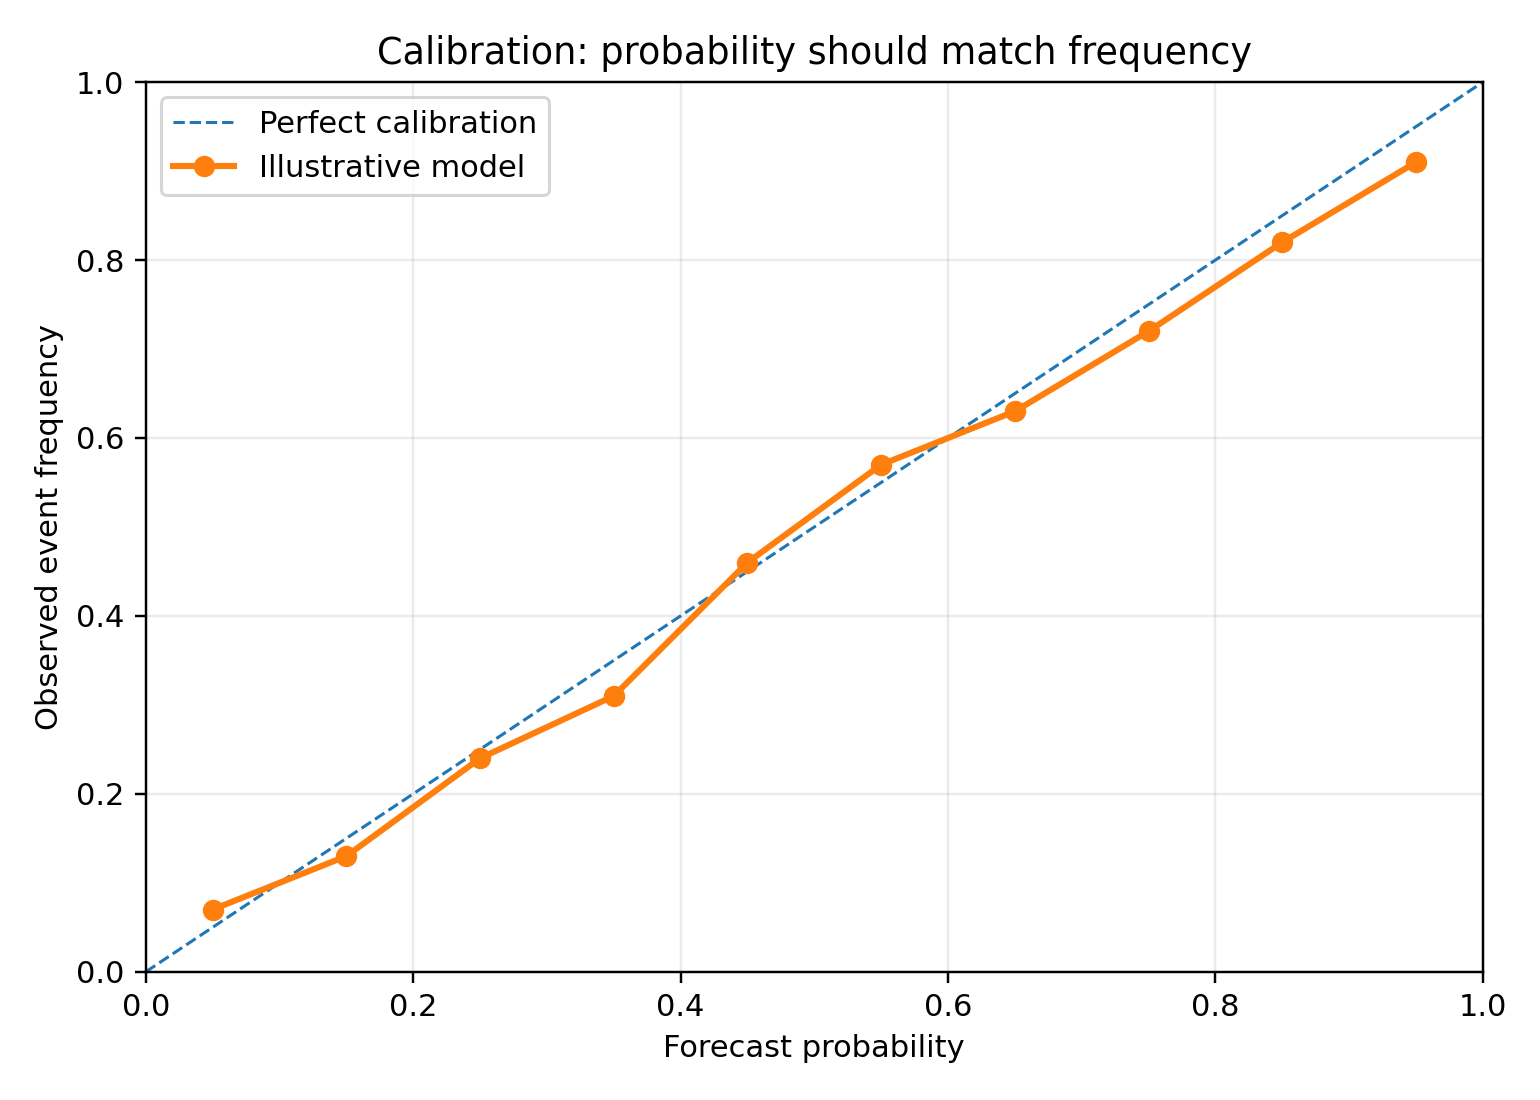
\includegraphics[width=0.75\textwidth]{calibration.png}
\caption{Illustrative probability calibration. A probability becomes useful when repeated forecasts at a given level occur at a similar frequency.}
\end{figure}

A probability is not a score out of 100. It is a statement about uncertainty \citep{gneiting2007calibration,gneiting2007proper}. A 60\% Forecast does not mean ``60\% good,'' and it does not mean the stock will rise 60\%. It means the model assigns a 0.60 probability to the exact event written on the Forecast card.

If the event is ``outperform the S\&P 500 over 12 months,'' then the model is comparing two future returns. The stock can lose money and still outperform if the benchmark loses more. The stock can rise and still underperform if the benchmark rises more.

\subsection{Why 50 percent matters}
For a balanced binary event, 50\% is the even-odds line. Being above 50\% means the model leans toward the event; being below 50\% means it leans away. How far the probability is from 50\% is not the same as how strong the model evidence is. A weak model can produce 70\%; evidence strength tells you whether that confidence has been supported historically.

\section{Evidence Strength: Probability and Evidence Are Different Axes}
Think of every Forecast as having two coordinates:
\begin{enumerate}[itemsep=0.2em]
\item the probability itself;
\item the evidence behind the model that produced it.
\end{enumerate}
A Limited-evidence probability should not be treated the same way as an identically sized probability from a research-validated model. That is why FinCompass displays both.

\begin{longtable}{p{0.20\textwidth}p{0.34\textwidth}p{0.36\textwidth}}
\toprule
Evidence & Plain meaning & Practical interpretation\\
\midrule
Limited & The probability model is valid enough to use as a reference, but stronger predictive improvement has not been established. & Useful for orientation and monitoring; interpret cautiously.\\
Research validated & The model passed stronger protected historical tests on its declared research corpus. & Stronger evidence, still limited to its market/horizon/data contract.\\
Market validated & Stronger validation plus stronger historical-universe and provenance controls. & Highest supported evidence tier; still not a guarantee.\\
\bottomrule
\end{longtable}

\section{Why This Ticker Can Use a Model It Was Not Trained On}
FinCompass uses pooled model families. This is similar to how a medical risk model can be trained on many people and then applied to a new patient who was not in the training data, provided the new case belongs to the population for which the model was designed.

For a stock model, the applicability contract might say: US common stock, US large-cap benchmark family, monthly features, 12-month horizon. If a newly entered ticker fits that domain and the required features can be constructed, it is an inference case. It is not a request to train a new model from scratch.

What should not happen is silent domain expansion. A US common-stock model should not automatically be used for a cryptoasset, bond ETF, commodity future, or foreign security merely because a price series exists.

\section{Why Model Updates Should Not Block a Working Forecast}
There are two separate questions:
\begin{quote}
Can the current model produce a scientifically valid Forecast?\\
Would it be useful to maintain or retrain the model on newer matured data?
\end{quote}
A model may be old and still be the best installed applicable model. In that case FinCompass should show the Forecast and separately indicate that maintenance is available. If a retraining attempt fails, the old model should remain intact.

This is similar to updating navigation maps: an available update does not necessarily mean the current map is unusable, and a failed update should not delete the map you already have.

\section{Three Kinds of Freshness}
\subsection{Ticker data freshness}
This answers: ``Do I have recent enough data to calculate today's features?''

\subsection{Model training freshness}
This answers: ``How old is the family corpus used when this model was fitted?''

\subsection{Retrainability}
This answers: ``Have enough new outcomes actually matured to make a retraining attempt meaningful?''

These are different. A ticker can have today's price while a 12-month label from six months ago is still immature. Therefore a data update can improve current analysis without creating new supervised outcomes.

\section{Start Live: What the Button Really Does}
\begin{figure}[H]
\centering
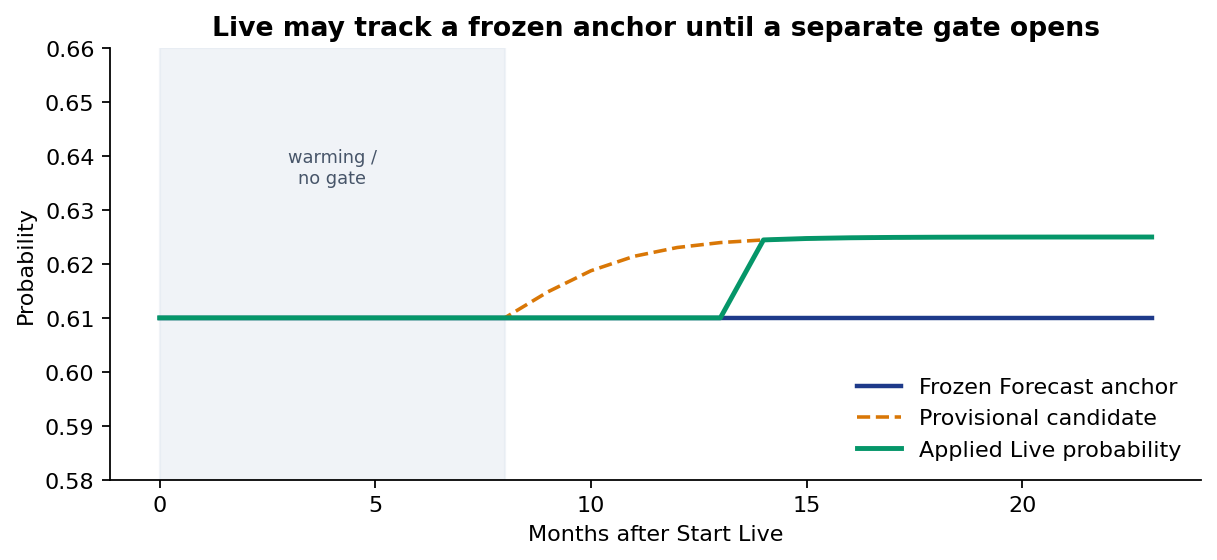
\includegraphics[width=0.92\textwidth]{live_residual.png}
\caption{Live starts from a frozen anchor. A Limited-evidence model stays tracking-only. A stronger model may apply a small residual only after a separate gate opens.}
\end{figure}

The user should only need one button, but FinCompass may choose one of two safe internal modes.

\subsection{Tracking-only Live}
Used for a Limited-evidence baseline. The original probability is monitored but there is no adaptive learning. This is still valuable because it provides one place to watch freshness, current context, and the original Forecast.

\subsection{Governed adaptive Live}
Used only when the anchor model is eligible and the adaptive layer has itself accumulated sufficient matured evidence. Fresh information may produce a candidate adjustment, but the candidate is not automatically applied.

\subsection{What you should see}
A good Live screen should answer:
\begin{itemize}[itemsep=0.15em]
\item What was the original Forecast?
\item What probability is currently being applied?
\item Is a provisional candidate different?
\item Is the adaptive layer active, warming, or degraded?
\item Why?
\end{itemize}
No user should have to understand an internal gate enum to answer those questions.

\section{Understanding Calibration Without Statistics Training}
\begin{figure}[H]
\centering
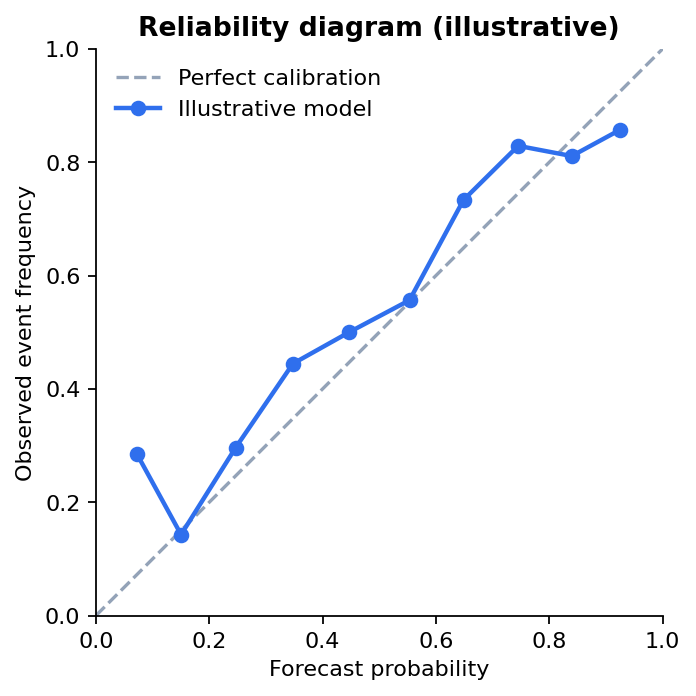
\includegraphics[width=0.55\textwidth]{reliability_diagram.png}
\caption{Illustrative reliability diagram. Points near the diagonal mean forecast probabilities roughly match observed frequencies \citep{gneiting2007calibration}.}
\end{figure}

Imagine a weather service makes one hundred 70\% rain forecasts over several years. If rain occurs on about seventy of those occasions, the forecasts are well calibrated at that level. If it rains only thirty times, the service is overconfident.

The same idea applies to FinCompass. Calibration asks whether probabilities behave like probabilities across historical cases. It does not ask whether the model ranks stocks perfectly, and it does not guarantee that the next 70\% Forecast will succeed.

\section{Understanding Brier Skill}
\begin{figure}[H]
\centering
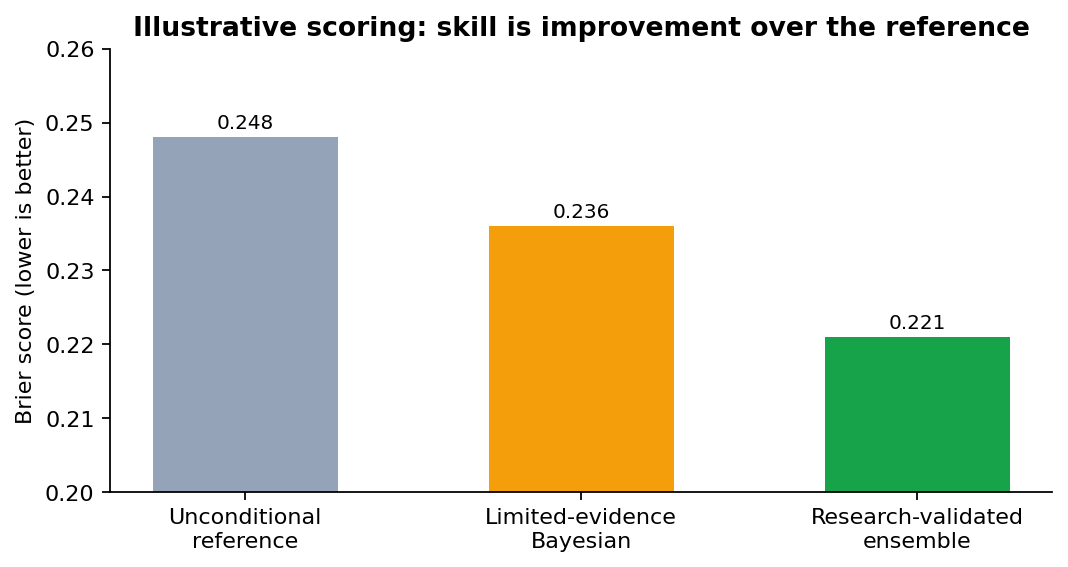
\includegraphics[width=0.78\textwidth]{brier_skill.png}
\caption{Illustrative Brier scores. Skill is improvement versus an unconditional reference, not a raw score in isolation \citep{brier1950verification,gneiting2007proper}.}
\end{figure}

Brier score measures probability error. If an event happens ($y=1$) and the model predicted $p=0.8$, the squared error is $(0.8-1)^2=0.04$. If the model predicted 0.2, the error is $(0.2-1)^2=0.64$. Confident wrong predictions are therefore costly.

Brier skill compares the model with a reference. A value of zero means the model did not improve the reference Brier score. Positive is better. Negative means the model's probabilities were worse than the reference on that evaluation set.

\section{Understanding Log Loss}
Log loss is another probability score. It is especially unforgiving when a model assigns a very small probability to something that then occurs. This is useful because a forecasting system should be cautious about extreme confidence unless the evidence truly supports it.

A model can have acceptable Brier score and still have poor log loss if a small number of highly confident misses dominate. Research mode therefore reports both.

\section{Understanding ROC AUC}
AUC asks a ranking question: if you randomly pick one historical case where the event happened and one where it did not, how often did the model assign the higher score to the event case? An AUC of 0.5 is roughly chance ranking. AUC does not tell you whether a displayed 70\% probability should really occur 70\% of the time. That is calibration's job.

\section{Why the Test Is Locked}
A model developer can make almost any backtest look better by repeatedly changing features and settings after looking at the test result \citep{white2000reality,harvey2016crosssection,bailey2017pbo}. The locked test exists to stop that behavior.

The process should be:
\begin{quote}
Train $\rightarrow$ development/validation decisions $\rightarrow$ freeze choices $\rightarrow$ open locked test once.
\end{quote}

\begin{figure}[H]
\centering
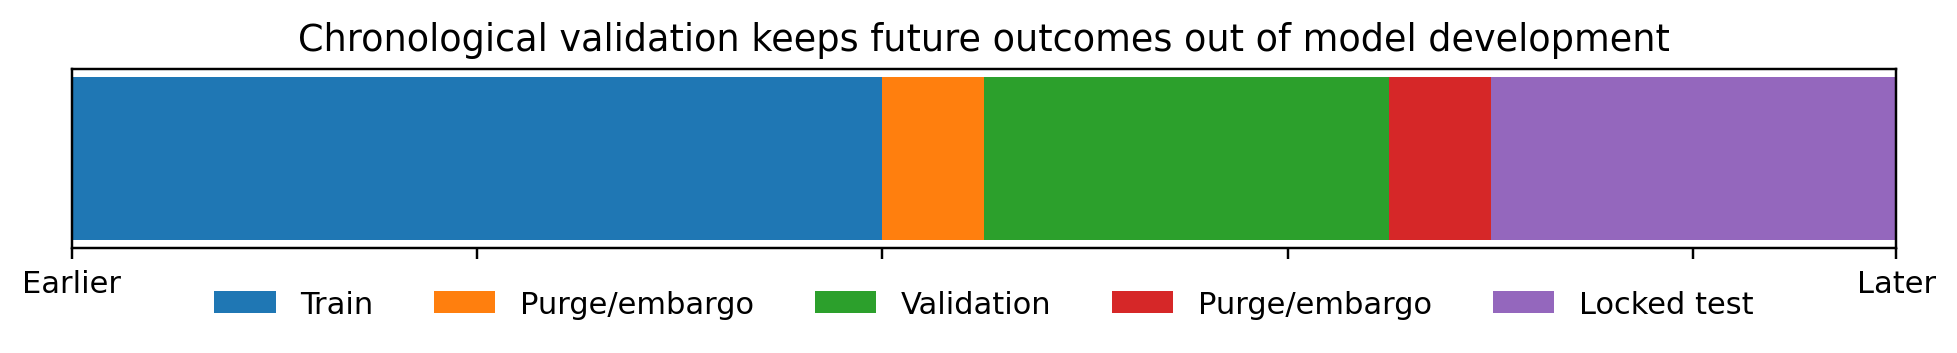
\includegraphics[width=0.94\textwidth]{temporal_split.png}
\caption{Illustrative protected chronological structure. The locked test is later in time and is not used to decide the model.}
\end{figure}

\section{Why Overlapping Horizons Matter}
Suppose you create a new 12-month Forecast every month. The January and February outcomes share eleven months of future market history. They are not independent coin tosses. If a backtest treats each row as independent, confidence intervals can become unrealistically narrow.

FinCompass therefore uses time-aware splitting and dependence-aware uncertainty methods. You do not need to calculate these yourself, but an expert should be able to inspect the method in Research Details.

\section{Understanding Regimes}
A regime is a hidden market state inferred from observable market behavior. It is not a label such as ``bull market'' typed by a developer after seeing the outcome. A hidden Markov model estimates the probability of being in each state using variables such as benchmark return and volatility.

The important safeguard is filtering: when asking what regime was believed to exist on a historical date, the model must use information available only through that date. Looking at future data to relabel the past would make the historical test optimistic.

\section{The Model Ladder}
\begin{figure}[H]
\centering
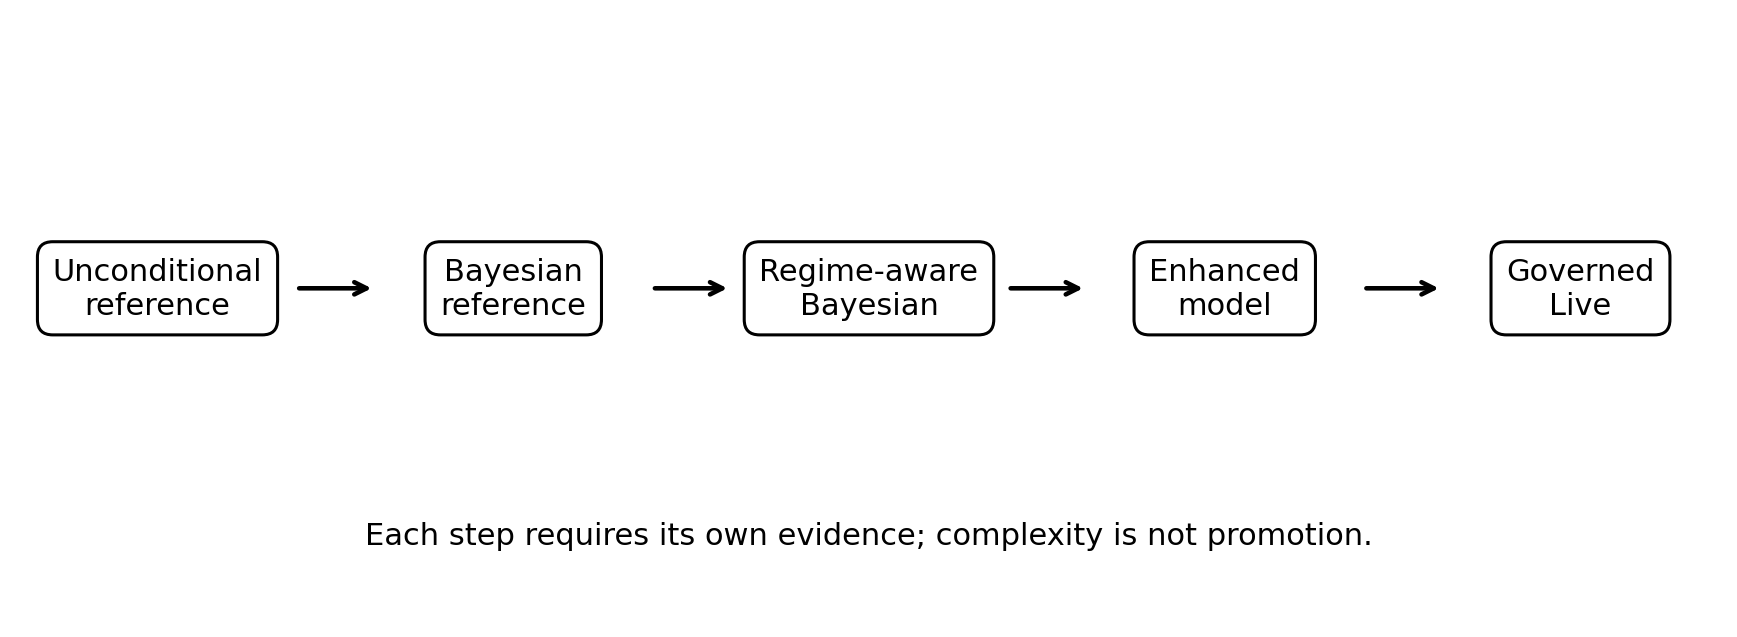
\includegraphics[width=0.90\textwidth]{model_ladder.png}
\caption{FinCompass model ladder. More complicated models are not automatically better.}
\end{figure}

The unconditional reference asks, ``How often did the event happen historically?'' The Bayesian reference asks whether a small set of backward-looking features improves that estimate. The regime model asks whether market state adds useful information. The enhanced model allows more nonlinear behavior. Each step has to demonstrate incremental value; complexity alone is not a reason to promote a model.

\section{DCF: From Cash Flow to an Estimated Value Range}
DCF asks a simple economic question with difficult assumptions: if this company generates cash in the future, what are those future cash flows worth today?

The current FinCompass DCF begins from reported free cash flow when available. It uses a multi-year base when possible so one unusual year does not dominate the whole valuation. Growth is anchored to the company's own historical free-cash-flow growth where the history is usable, with revenue growth as a fallback.

The forecast uses three stages: an early growth stage, a transition stage, and a stable terminal stage. The stable rate is capped because no mature company can outgrow the entire economy forever.

\begin{figure}[H]
\centering
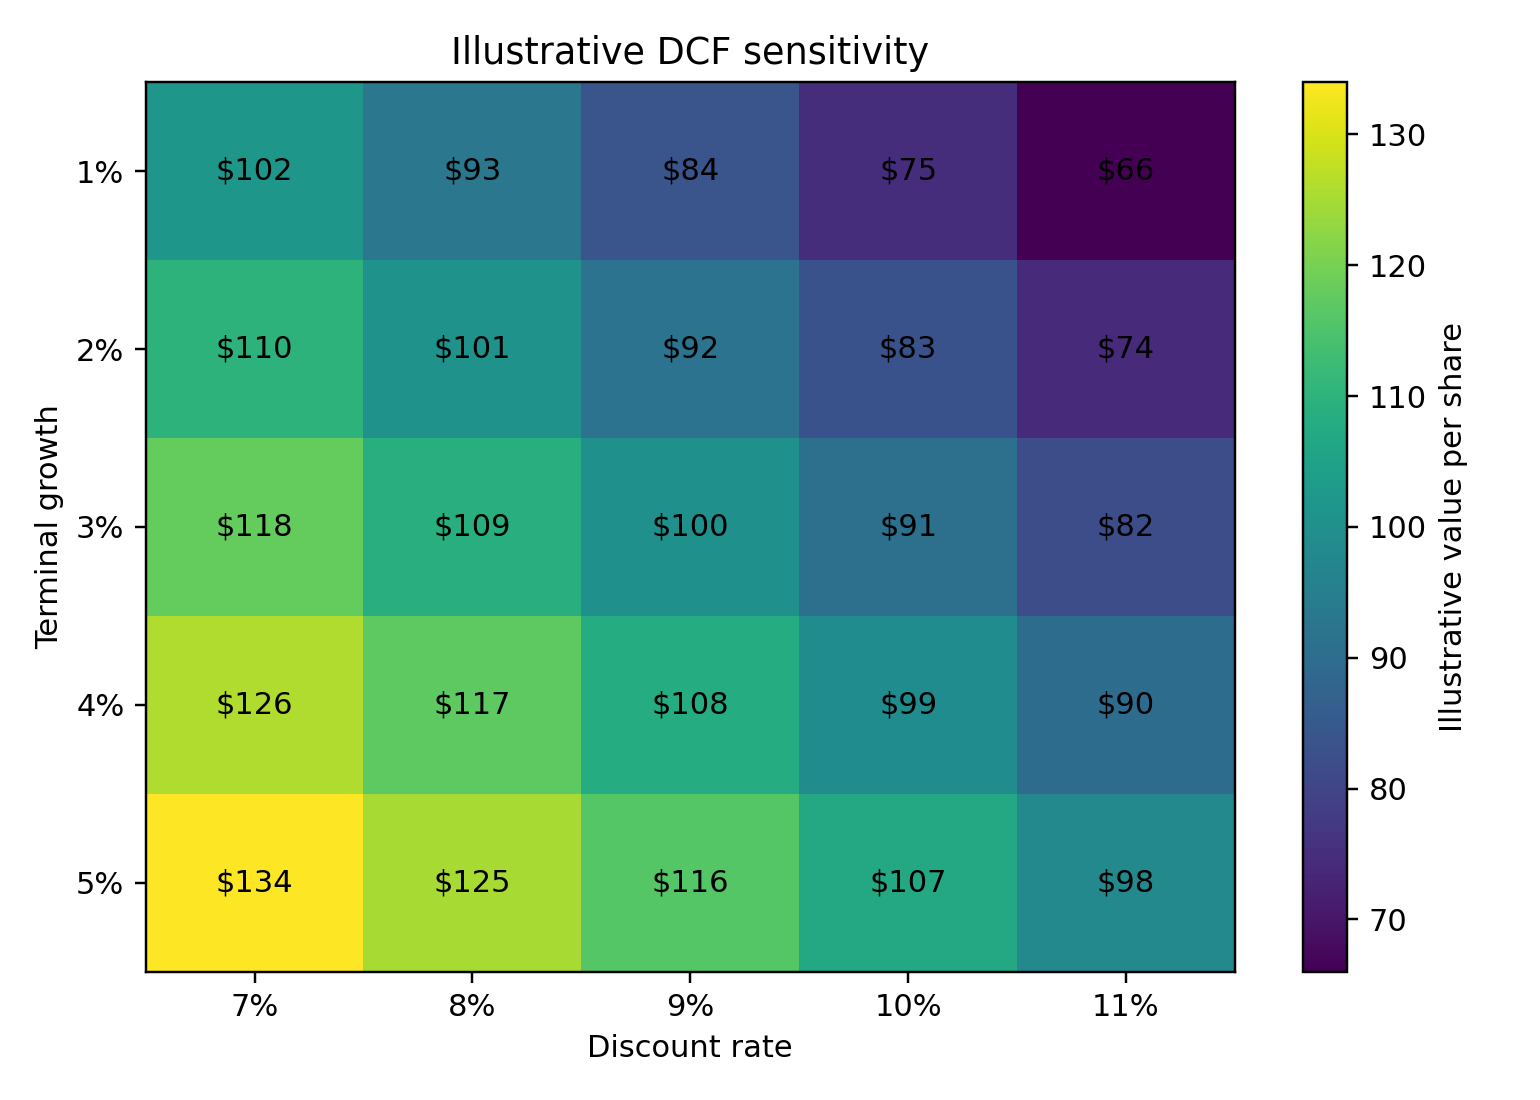
\includegraphics[width=0.76\textwidth]{dcf_sensitivity.png}
\caption{Illustrative sensitivity. DCF is a range of outcomes under assumptions, not a single objectively true price.}
\end{figure}

\subsection{How to read a fair-value gauge}
If the current price is inside the estimated range, the simplest interpretation is that the market price is broadly consistent with the modeled assumptions. If the price is far above the range, that does not prove the stock is ``wrong.'' It can mean the market expects faster growth, better margins, a lower risk premium, or other economics not assumed by the model.

\subsection{Reverse DCF}
Reverse DCF starts with today's price and asks what growth rate would make the cash-flow model justify it. This is useful because the question becomes concrete: ``The current price appears to require approximately X\% early-stage FCF growth under the remaining assumptions. Is that expectation plausible?''

\section{Options: Reading the Contract Before the Greeks}
The options desk now uses the analyzed ticker and can load real listed contracts when the public feed is available. The first questions should be practical:
\begin{enumerate}[itemsep=0.15em]
\item Is this a call or put?
\item What is the strike?
\item How many days remain?
\item What premium is quoted?
\item Where is break-even at expiry?
\item What is the maximum loss for this long-option example?
\end{enumerate}
Only after those questions are clear do Delta, Gamma, Vega, Theta, and Rho become useful.

\begin{figure}[H]
\centering
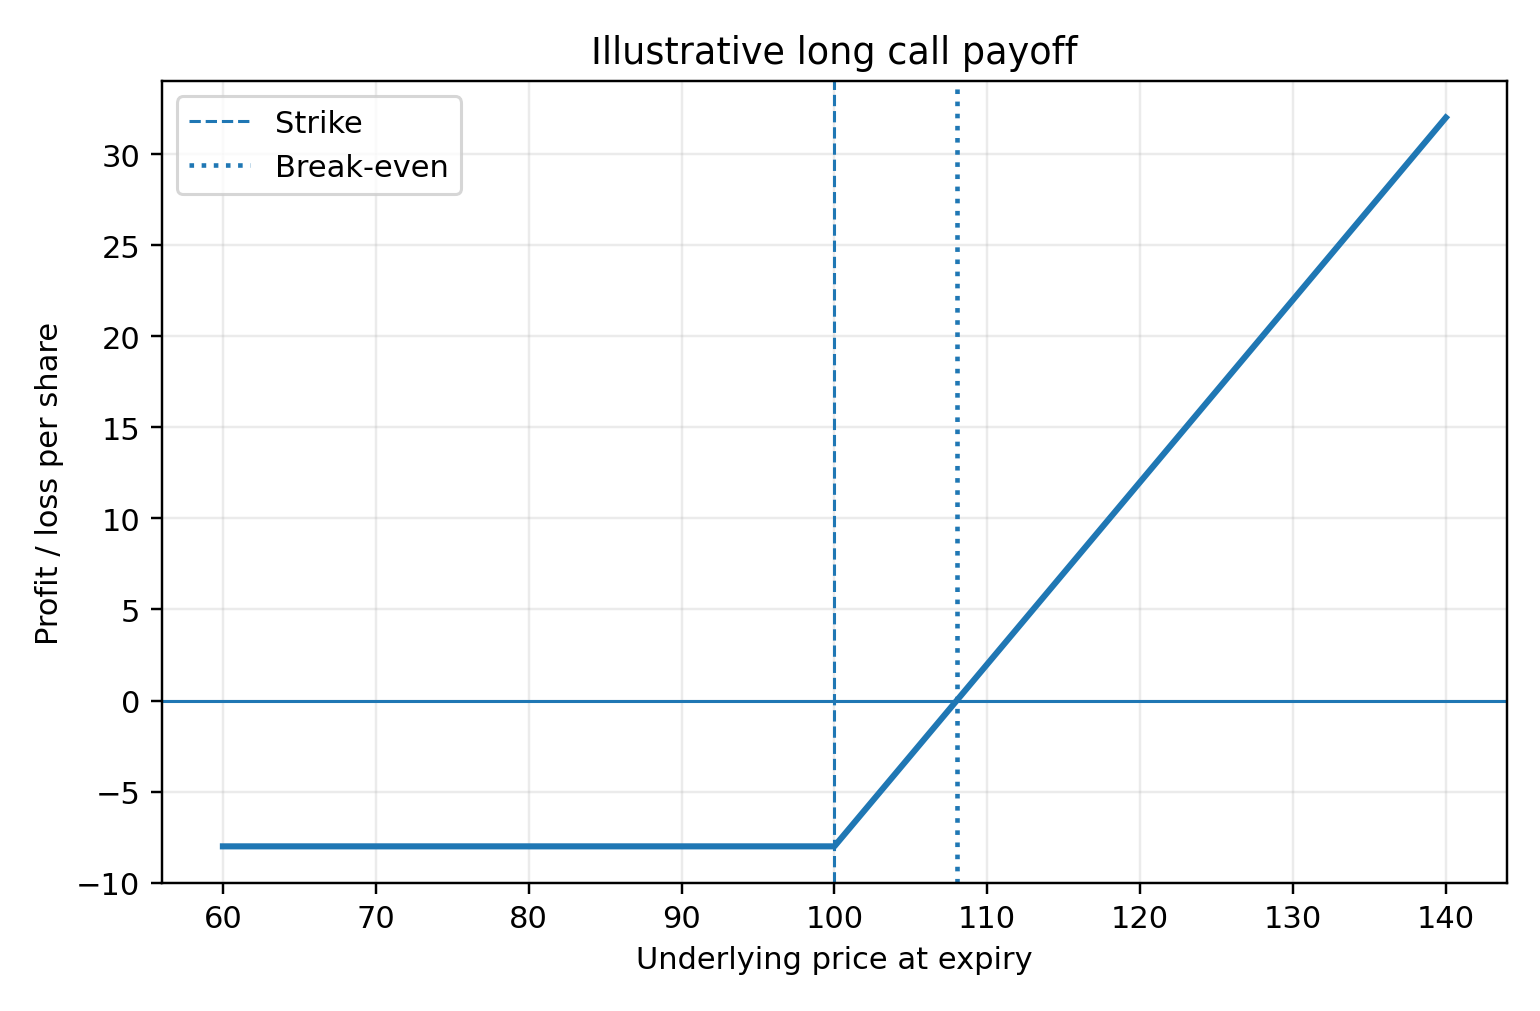
\includegraphics[width=0.76\textwidth]{option_payoff.png}
\caption{Illustrative long call. Below break-even the position loses money at expiry; loss is capped at the premium for a simple long call.}
\end{figure}

\subsection{ITM, ATM, and OTM}
In-the-money (ITM) means the option already has intrinsic value. At-the-money (ATM) means the strike is near the current underlying price. Out-of-the-money (OTM) means exercise would not currently create intrinsic value. These labels describe moneyness, not whether a contract is ``good'' or ``bad.''

\subsection{LEAPS}
LEAPS are long-dated listed options, commonly with a year or more remaining. More time reduces immediate time pressure but usually increases premium. Long-dated options are still sensitive to implied volatility, dividends, rates, and the underlying price path.

\section{Bonds and the Treasury Curve}
The Treasury curve is a reference for current risk-free-ish government yields across maturities. It is useful context, but it is not automatically the right yield for a corporate bond. Corporate yields normally include additional compensation for credit and liquidity risk.

Bond price moves inversely with yield. Duration estimates how sensitive price is to a small yield change. Convexity improves the approximation for larger changes. Call features, default risk, and spread changes require additional analysis.

\section{Portfolio Risk: Weight Is Not Risk}
A portfolio with four 25\% positions does not necessarily have four equal risk contributions. A more volatile holding, or one highly correlated with the rest, can dominate total portfolio variability.

\begin{figure}[H]
\centering
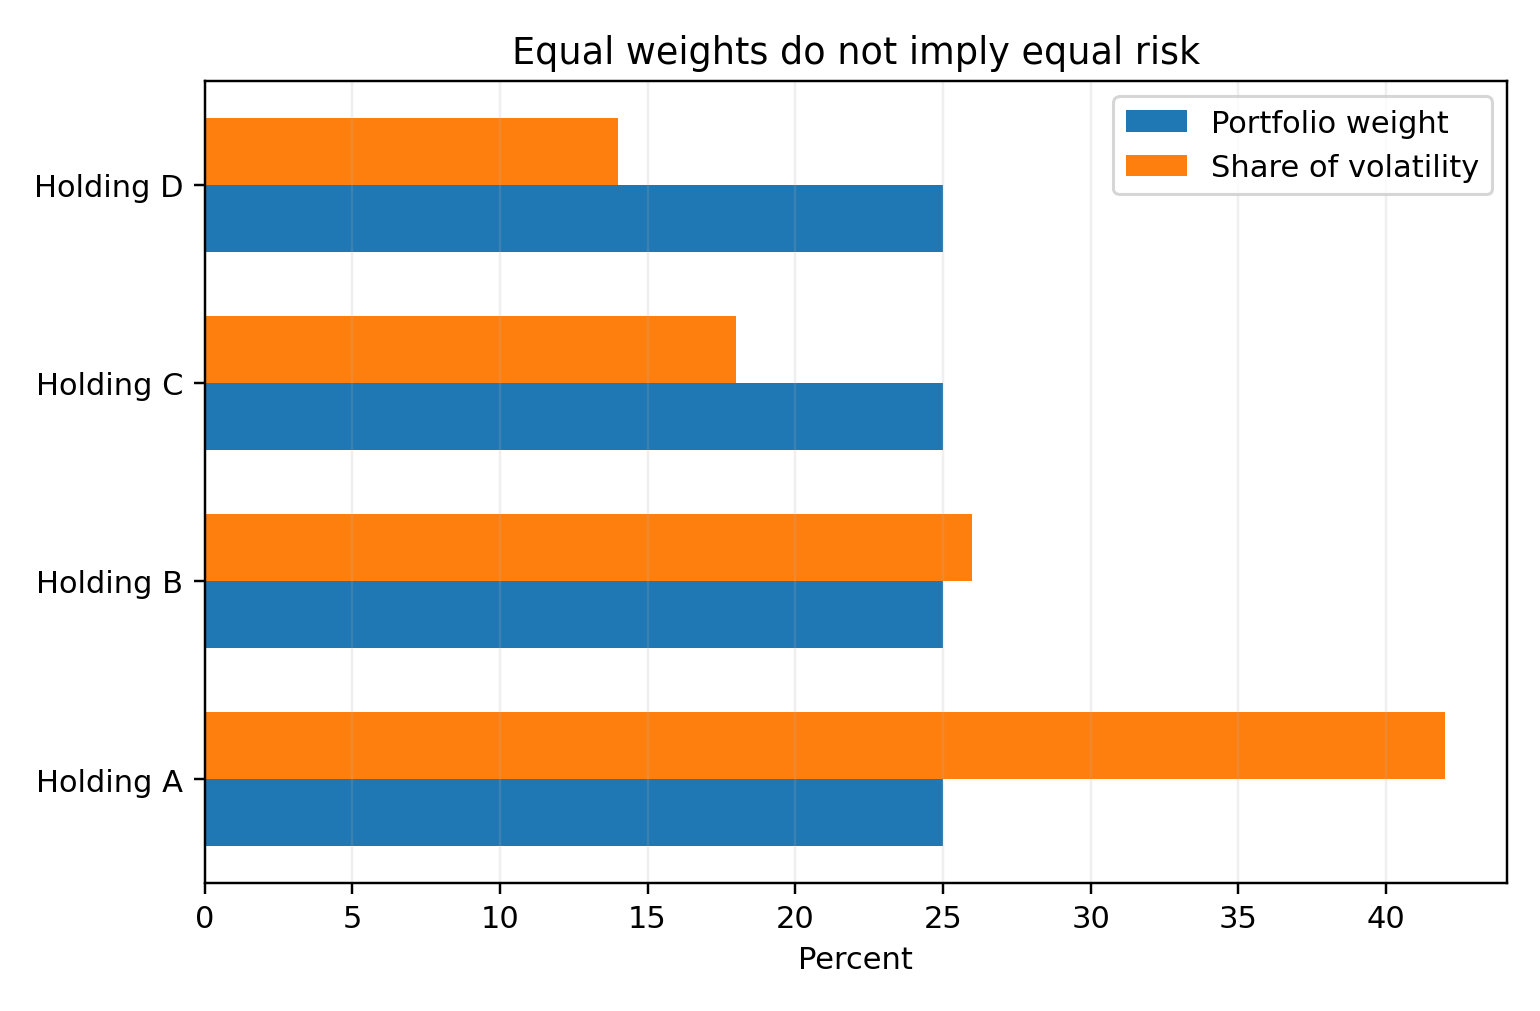
\includegraphics[width=0.72\textwidth]{portfolio_risk.png}
\caption{Illustrative equal-weight portfolio in which one holding contributes much more than one-quarter of total volatility.}
\end{figure}

The most useful plain-language question is: ``Which holding is driving the portfolio's movement?'' Research Details can then show the covariance matrix, volatility assumptions, and risk-contribution calculation.

\section{Drawdown: The Number Many Users Understand Immediately}
Volatility can feel abstract. Drawdown is often more intuitive. If an investment rises to $100 and later falls to $70 before recovering, the drawdown from that peak is 30\%.

\begin{figure}[H]
\centering
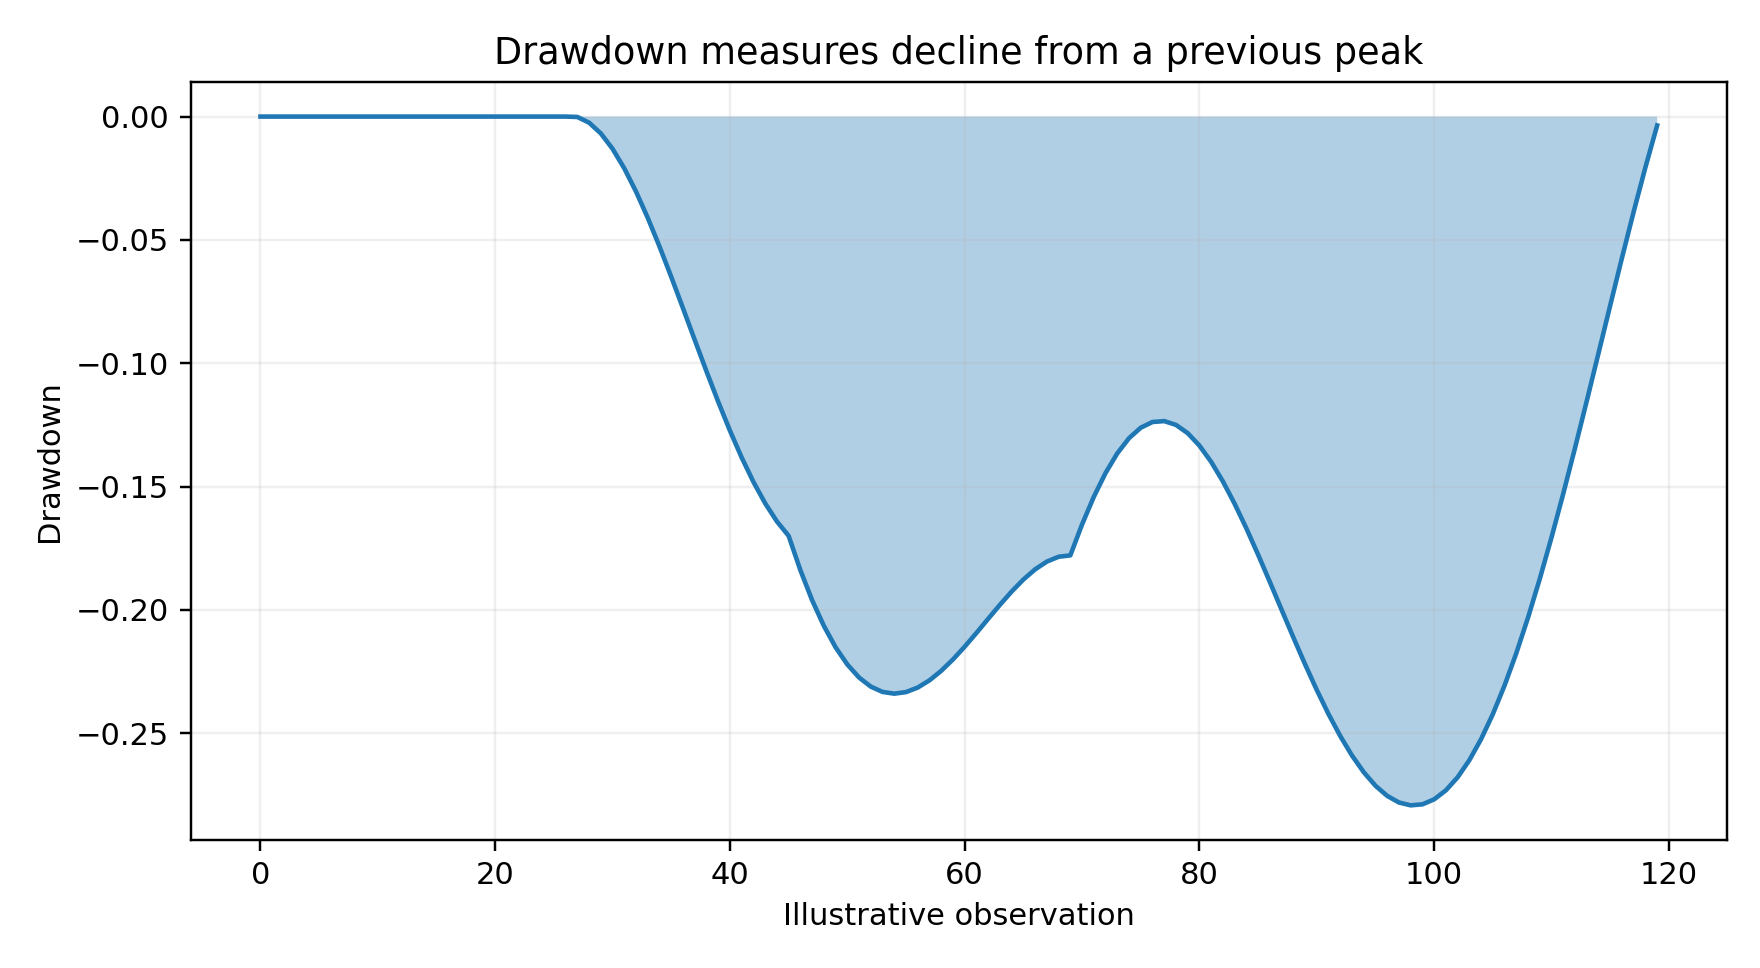
\includegraphics[width=0.78\textwidth]{drawdown.png}
\caption{Illustrative drawdown path. Maximum drawdown is the worst historical peak-to-trough decline in the selected period.}
\end{figure}

Maximum drawdown is not a worst-case guarantee. The future can be worse than the historical sample.

\section{Sharpe and Sortino in Plain Language}
Sharpe asks how much historical excess return was obtained per unit of total volatility. Sortino uses downside deviation instead of all volatility. A higher ratio can be useful, but it can be inflated by a favorable sample period, stale prices, smoothing, or a strategy that hides rare tail losses. Always read it with drawdown and tail measures.

\section{VaR and Expected Shortfall}
A 95\% one-day VaR is approximately a threshold that historical/model losses exceeded about 5\% of the time under the stated method. It is not the maximum possible loss. Expected shortfall asks: when losses were beyond that threshold, how large were they on average?

The method matters. Historical, parametric, and volatility-filtered estimates can differ. Research mode should identify which one FinCompass used.

\section{Financial Statements: Why Normalization Matters}
Data providers often use different names for the same accounting concept. One may say ``Total Revenue,'' another ``Operating Revenue.'' FinCompass maps provider vocabulary to canonical fields before formulas are applied.

Missing stays missing. A missing debt field is not silently treated as zero debt. That distinction is fundamental because otherwise ratios can look excellent simply because data were absent.

\section{Ratio Interpretation Cards}
\begin{longtable}{p{0.19\textwidth}p{0.30\textwidth}p{0.42\textwidth}}
\toprule
Ratio & Plain meaning & Important caution\\
\midrule
Gross margin & Share of revenue remaining after direct cost of goods/services. & Sector business models differ dramatically.\\
Operating margin & Share of revenue remaining after operating expenses. & Restructuring and classification choices can distort comparisons.\\
Net margin & Net income as a share of revenue. & Tax and one-time items can dominate.\\
ROE & Profit relative to shareholder equity. & Negative or very small equity can make ROE misleading.\\
ROIC & Operating return relative to invested capital. & Depends on capital-definition choices.\\
Current ratio & Current assets relative to current liabilities. & Not directly comparable across every industry.\\
Debt/equity & Debt relative to shareholder equity. & Negative equity can make the ratio economically awkward.\\
Interest coverage & Earnings/cash-flow capacity relative to interest expense. & Cyclical earnings can make a point estimate optimistic.\\
FCF margin & Free cash flow relative to revenue. & FCF can be temporarily distorted by working capital or capex cycles.\\
FCF yield & Free cash flow relative to market value. & A high yield can reflect genuine cheapness or deteriorating expectations.\\
\bottomrule
\end{longtable}

\section{Technical Indicators: Description, Not Destiny}
\begin{figure}[H]
\centering
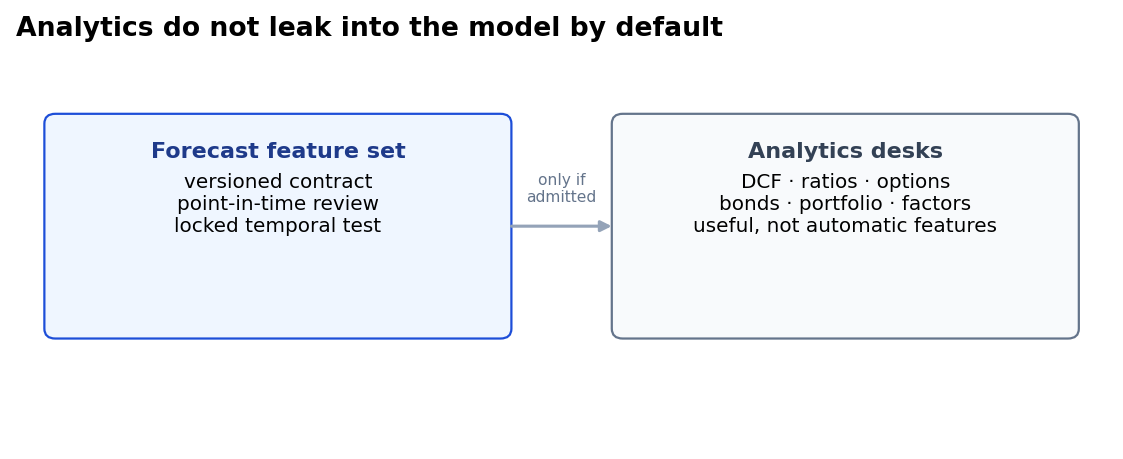
\includegraphics[width=0.92\textwidth]{feature_isolation.png}
\caption{DCF values, ratios, options and technicals stay on the analytics desks unless a versioned feature contract admits them into the Forecast model \citep{white2000reality,bailey2017pbo}.}
\end{figure}

RSI, MACD, moving averages, Bollinger Bands, and ATR describe properties of the recent price series. An RSI above 70 does not mathematically require the price to fall. A moving-average crossover does not guarantee a trend will continue. These indicators become Forecast features only if explicitly added to a feature contract and validated through the same protected process.

\section{Factor Regression: What Beta and Alpha Do and Do Not Mean}
A factor regression decomposes historical return variation into exposures to supplied factor-return series. Beta is an estimated sensitivity. Alpha is the intercept left after accounting for the included factors. A statistically significant historical alpha is not proof of a repeatable future opportunity; omitted factors, multiple testing, transaction costs, and regime changes can all matter.

R-squared describes how much in-sample variation the model explains. It is not a forecast-accuracy score.

\section{The Interpretation Policy: Useful, but Separate From the Model}
\begin{figure}[H]
\centering
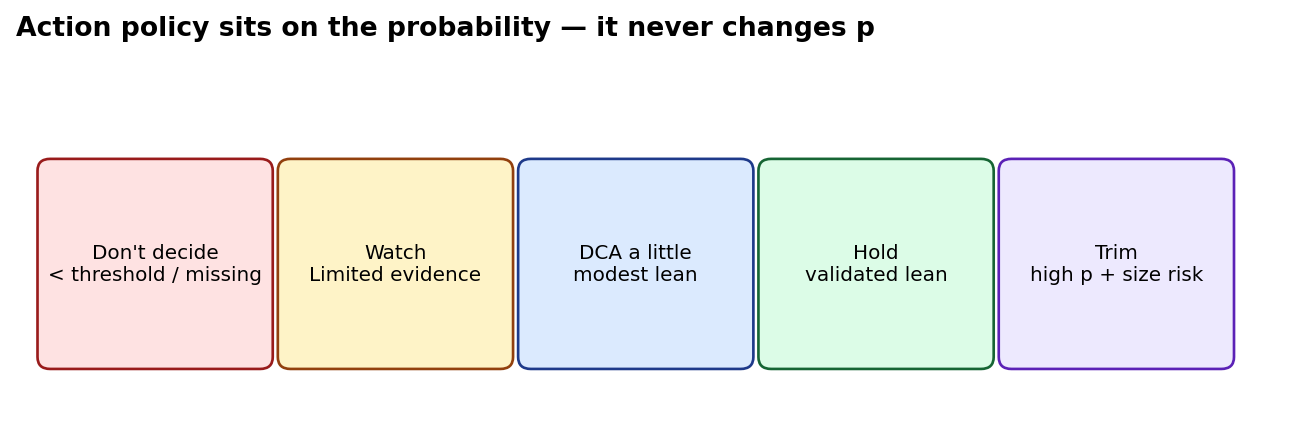
\includegraphics[width=0.98\textwidth]{action_policy.png}
\caption{The action policy maps probability and evidence tier onto at most five verbs. It never edits the Forecast $p$, never says ``buy all,'' and never auto-sizes a position.}
\end{figure}

FinCompass may display a practical posture such as Watch, Hold, DCA a little, or Trim. This layer is intentionally separate from the forecasting model. The probability is calculated first; the interpretation policy then maps the probability and evidence tier to a plain-language posture.

This distinction matters. A probability threshold is not a universal investment optimum. Personal tax situation, time horizon, current position, portfolio concentration, liquidity needs, and risk tolerance can change what action is appropriate. The policy should therefore be understood as a conservative educational interpretation rule, not personalized portfolio advice.

For professional presentation, source and interface language should use neutral, durable terminology. The product can be highly accessible without labeling its users.

\section{Why This Result?}
Every major output should eventually support a ``Why this result?'' explanation. For Forecast, it can say:
\begin{quote}
FinCompass used the 12-month US-equity family because this instrument is a US common stock, the model benchmark is the S\&P 500 family, the required history was available, and this was the strongest installed model matching the domain and horizon.
\end{quote}
For an unavailable Forecast:
\begin{quote}
FinCompass can analyze this instrument, but none of the installed Forecast model families is validated for this asset type and market.
\end{quote}
This is far more useful than exposing an internal rejection code.

\section{Troubleshooting Decision Tree}
\begin{enumerate}[itemsep=0.35em]
\item \textbf{No Forecast?} Check whether the instrument is supported and whether an applicable horizon/model family exists.
\item \textbf{Data unavailable?} Use Update data; if the provider is unavailable, keep the analytical limitation visible rather than substituting invented values.
\item \textbf{Model update unavailable?} The current model may be Forecast-only or the family retrainer may not exist. The current Forecast should remain intact.
\item \textbf{Model update failed?} Keep the previous model; inspect the Research diagnostic only if needed.
\item \textbf{Live shows no change?} Determine whether you are in tracking-only mode or the adaptive layer is still warming.
\item \textbf{DCF looks far from market price?} Inspect base FCF, growth path, discount rate, terminal growth, and reverse-DCF implied growth before concluding the market is mispriced.
\item \textbf{Option result seems unrealistic?} Check whether the displayed premium is a real delayed quote, whether bid--ask spread is wide, and whether the model assumptions match the contract.
\end{enumerate}

\section{A Complete Worked Example: New Ticker to Live}
Assume you enter a valid US common stock that was not one of the model's training symbols.

\subsection{1. Identification}
FinCompass resolves the ticker and identifies it as a US common stock. It assigns the US large-cap benchmark family. If classification fails, Forecast stops before any model is applied.

\subsection{2. Model selection}
The registry finds model families matching asset class, region, security type, monthly frequency, and requested horizon. If a research-validated 12-month model is applicable, it should outrank a Limited-evidence baseline at the same contract. If only a baseline exists, the baseline can still produce a Forecast with the Limited evidence label.

\subsection{3. Feature construction}
The current ticker history and benchmark history are used to construct the model's exact backward-looking feature vector. The software does not retrain merely because the ticker is new.

\subsection{4. Forecast}
The result might be 57\%. Read the event before the number: ``57\% probability of outperforming the S\&P 500 over 12 months.'' Then read the evidence label.

\subsection{5. Freshness}
Ticker data may be current while the model's family training cutoff is older. That should appear as context, not a reason to erase the Forecast.

\subsection{6. Live}
Choose Start Live. If the model is a baseline, Live is tracking-only. If the model is an eligible validated anchor, the adaptive layer may still remain inactive until enough outcomes have matured.

\section{A Complete Worked Example: Reading a DCF}
Suppose the current price is \$120 and the displayed DCF range is \$95--\$135. Do not read this as ``the stock is worth exactly \$115.'' Read it as: under the model's current cash-flow normalization, growth path, discount-rate range, and terminal assumptions, a range spanning \$95--\$135 is produced.

Now inspect reverse DCF. If the current price implies 11\% early-stage FCF growth, ask whether the company's historical economics and competitive position make that expectation plausible. If your answer is yes, a market price above the base DCF may be understandable. If your answer is no, the gap deserves investigation. The purpose is disciplined assumption comparison, not a single-number verdict.

\section{A Complete Worked Example: Long Call}
Assume stock price \$100, call strike \$100, premium \$8. At expiry:
\begin{itemize}[itemsep=0.15em]
\item at \$90, the option expires worthless and the loss is the \$8 premium;
\item at \$100, the option still expires with no intrinsic value and the loss is \$8;
\item at \$108, intrinsic value is \$8 and the position is at break-even before fees;
\item at \$120, intrinsic value is \$20 and profit is \$12 before fees.
\end{itemize}
The Black--Scholes model value before expiry is a different concept because it includes remaining time value and model assumptions.

\section{A Complete Worked Example: Portfolio Concentration}
Suppose four holdings each have 25\% capital weight, but Holding A contributes 42\% of portfolio volatility. The correct conclusion is not that Holding A is ``bad.'' It is that the portfolio's movement is disproportionately sensitive to that holding. You may then investigate whether the concentration is intentional and whether correlations change in stress periods.

\section{Searchable Glossary Specification}
The application should include a dedicated searchable Glossary and Reference page with category filters such as Forecasting, Validation, Risk, Valuation, Options, Fixed Income, Portfolio, Statistics, and Data. Every common tooltip should link to the matching entry.

Each glossary entry should contain:
\begin{enumerate}[itemsep=0.15em]
\item Plain meaning;
\item Why it matters;
\item How FinCompass uses it;
\item Important limitation;
\item Formula or technical definition when useful.
\end{enumerate}

\section{Glossary: Forecasting and Validation}
\begin{longtable}{p{0.18\textwidth}p{0.74\textwidth}}
\toprule
Term & Reference explanation\\
\midrule
Forecast & A probability assigned to one precisely defined future event. Always read the benchmark, horizon, and event threshold together with the probability.\\
Benchmark & The comparison investment used by a relative-return Forecast. Outperforming the benchmark is different from simply earning a positive return.\\
Horizon & The future period over which the event is defined, such as 6, 12, 24, or 36 months. Different horizons are different targets.\\
Outperformance & Return greater than the benchmark return by more than the declared threshold over the same period.\\
Uncertainty range & Range reflecting uncertainty in the estimated probability under the model; it is not a range of possible stock returns.\\
Evidence strength & Label describing what level of validation/provenance has been established for the model.\\
Bayesian baseline & Hard-valid probability model available for Forecast when stronger predictive skill has not been established.\\
Research validated & Model that passed stronger protected historical validation on its declared corpus.\\
Market validated & Strongest tier, adding stronger market-universe and provenance controls.\\
Locked test & Final historical period protected from development decisions.\\
Calibration & Whether repeated stated probabilities correspond to similar observed frequencies.\\
Brier score & Squared probability error. Lower is better.\\
Brier skill & Improvement in Brier score versus a declared reference probability. Positive is better than the reference.\\
Log loss & Probability loss that strongly penalizes confident wrong forecasts. Lower is better.\\
ROC AUC & Ranking measure; 0.5 is roughly chance ranking and 1.0 is perfect ranking. It does not measure calibration.\\
ECE & Expected calibration error, a bin-based summary of the gap between predicted and observed frequencies.\\
Walk-forward validation & Repeated chronological evaluation as the development window moves through time.\\
Bootstrap & Resampling method used to estimate uncertainty. Financial time dependence requires block/date-aware designs rather than naive row resampling.\\
Purge & Removal of rows whose forward outcome overlaps a later partition.\\
Embargo & Additional time gap between partitions.\\
Matured label & Outcome whose original forecast horizon has completed and can now be used for evaluation or learning.\\
Applicability domain & Declared market/security/horizon conditions under which a model is allowed to be used.\\
\bottomrule
\end{longtable}

\section{Glossary: Risk and Performance}
\begin{longtable}{p{0.18\textwidth}p{0.74\textwidth}}
\toprule
Term & Reference explanation\\
\midrule
Annualized return & Compounded historical return converted to an annual rate for comparison. It does not imply the future will repeat.\\
Volatility & Historical dispersion of returns, often annualized. It measures variability, not direction.\\
Sharpe ratio & Historical excess return per unit of total volatility. Sensitive to sample period and return distribution.\\
Sortino ratio & Return relative to downside deviation, focusing on unfavorable variability.\\
Drawdown & Decline from a previous running peak.\\
Maximum drawdown & Largest historical peak-to-trough decline in the selected sample. Not a worst-case guarantee.\\
Beta & Estimated historical sensitivity to benchmark movements. Can change over time.\\
Tracking error & Volatility of active return relative to a benchmark.\\
VaR & Estimated loss quantile under a declared method and horizon. It is not the maximum possible loss.\\
Expected shortfall & Average loss conditional on being beyond a VaR threshold under the chosen method.\\
Correlation & Standardized measure of co-movement. Correlations can rise in stress.\\
Covariance & Joint variability used in portfolio variance calculations.\\
Risk contribution & Approximate share of total portfolio volatility attributable to each position under the covariance model.\\
\bottomrule
\end{longtable}

\section{Glossary: Valuation and Financial Statements}
\begin{longtable}{p{0.18\textwidth}p{0.74\textwidth}}
\toprule
Term & Reference explanation\\
\midrule
Free cash flow & Cash generated after operating needs and capital expenditure under the declared definition. Different providers may define it differently.\\
DCF & Discounted cash-flow valuation: present value of assumed future cash flows plus terminal value. Highly assumption sensitive.\\
Discount rate & Required return used to translate future cash flows into present value. Higher rates reduce present value.\\
WACC & Weighted average cost of capital, commonly used for unlevered enterprise-value DCFs.\\
Terminal growth & Long-run growth assumption used in a perpetual-growth terminal value. Must remain below the discount rate and economically plausible.\\
Reverse DCF & Calculation of the growth assumption implied by the current market price under other fixed assumptions.\\
Revenue CAGR & Compound annual growth rate of revenue over a historical interval.\\
FCF CAGR & Compound annual growth rate of free cash flow; can be unstable when endpoints are small or negative.\\
Gross margin & Gross profit divided by revenue.\\
Operating margin & Operating income divided by revenue.\\
ROE & Net income relative to shareholder equity. Can be misleading with negative or unusually small equity.\\
ROIC & Return generated relative to invested capital under the formula's capital definition.\\
Current ratio & Current assets divided by current liabilities.\\
Debt/equity & Debt relative to shareholder equity. Negative equity complicates interpretation.\\
Interest coverage & Earnings or cash-flow measure relative to interest expense.\\
\bottomrule
\end{longtable}

\section{Glossary: Options and Fixed Income}
\begin{longtable}{p{0.18\textwidth}p{0.74\textwidth}}
\toprule
Term & Reference explanation\\
\midrule
Call & Option giving the holder the right, not obligation, to buy under the contract terms.\\
Put & Option giving the holder the right, not obligation, to sell under the contract terms.\\
Strike & Contract price used to determine exercise value.\\
Premium & Price paid/received for the option contract. Market premium and model value can differ.\\
Break-even & Underlying price at expiry where a simple long-option position has zero profit before fees.\\
Implied volatility & Volatility input that makes an option-pricing model match a market price. It is model dependent and varies by strike/expiry.\\
Delta & First-order sensitivity of option value to a small underlying-price change under the pricing model.\\
Gamma & Sensitivity of Delta to the underlying price.\\
Vega & Sensitivity of option value to implied volatility.\\
Theta & Sensitivity of option value to passage of time, holding other model inputs fixed.\\
Rho & Sensitivity of option value to interest rates.\\
ITM & In-the-money; the option currently has intrinsic value.\\
ATM & At-the-money; strike is near the underlying price.\\
OTM & Out-of-the-money; the option currently has no intrinsic exercise value.\\
LEAPS & Long-dated listed options, commonly with at least about one year to expiry.\\
Yield curve & Yields across maturities for a given issuer/class, such as US Treasuries.\\
Duration & First-order bond-price sensitivity to yield changes.\\
Convexity & Curvature adjustment improving duration's approximation for larger yield changes.\\
\bottomrule
\end{longtable}

\section{Glossary: Data, Models, and Live}
\begin{longtable}{p{0.18\textwidth}p{0.74\textwidth}}
\toprule
Term & Reference explanation\\
\midrule
Point-in-time data & Data aligned to when it was actually public/known, not merely to the fiscal period it describes.\\
Survivorship bias & Distortion caused by studying only securities that survived to the present.\\
Corporate action & Split, dividend, merger, spin-off, or similar event that can alter historical price/return interpretation.\\
Price basis & Convention such as raw close or adjusted close used for return calculations.\\
Model family & Forecasting architecture trained across a declared class of instruments.\\
Pooled model & Model trained on multiple securities and applied to new in-domain securities.\\
Feature contract & Exact versioned definition of model inputs and transformations.\\
Training contract & Runtime metadata declaring trainer family, recipe, feature contract, horizon, benchmark family, and retrainability.\\
Candidate model & Newly trained artifact awaiting evaluation/replacement decision.\\
Active model & Model currently designated for an adaptive Live role where activation is permitted.\\
Tracking-only Live & Monitoring mode with no adaptive residual learning/application.\\
Adaptive Live & Governed mode in which a validated anchor may receive a bounded residual after separate online evidence gates pass.\\
Pending label & Live observation waiting for its horizon to finish before its outcome can be learned.\\
Drift & Evidence that recent predictive loss behavior differs materially from the anchor/reference expectation.\\
Lineage & Record of parent model, recipe, settings, and replacement history.\\
Artifact hash & Cryptographic digest used to verify exact model bytes/manifest integrity.\\
\bottomrule
\end{longtable}

\section{Checklist: Before You Trust What You Are Looking At}
Before acting on any output, ask:
\begin{enumerate}[itemsep=0.2em]
\item Am I reading a Forecast, an evidence score, a valuation, or a historical statistic?
\item What benchmark and horizon apply?
\item What is the evidence strength?
\item Is the instrument inside the model's applicability domain?
\item Are the data current enough for this analysis?
\item Is the model itself older, and if so, is that merely maintenance context or a hard limitation?
\item Are the important assumptions visible?
\item Would a small change in assumptions materially change the conclusion?
\item Is the result descriptive, probabilistic, or prescriptive?
\item If an interpretation/action label is shown, am I treating it as a general policy rather than personalized advice?
\end{enumerate}

\section{What the Software Should Still Improve}
The current implementation has made major usability progress, but several improvements would make the layman-to-expert bridge stronger:
\begin{itemize}[itemsep=0.2em]
\item add the dedicated searchable Glossary and Reference page in the application;
\item link every major tooltip to its glossary entry;
\item add a ``Why this result?'' disclosure for model selection, DCF interpretation, and unavailable Forecasts;
\item keep model/data/retrain freshness separate in the visible UI;
\item expose timestamps and source labels for option-chain and Treasury data;
\item keep source and interface terminology professional and durable;
\item show raw DCF scenario values in Research when the Guided display uses a bounded/trimmed visual range;
\item complete a packaged Forecast-to-Live persistence test and make its evidence part of release verification;
\item add a printable/exportable Forecast evidence report for expert review without exposing private modeling intermediates.
\end{itemize}


\setcounter{section}{0}
\renewcommand{\thesection}{\arabic{section}}

\clearpage
\part{Detailed Glossary and Mini-Reference}
\section{How to Read the Glossary}
The entries below are intentionally longer than a tooltip. A tooltip should answer ``what is this?'' in one or two sentences. This mini-reference answers five questions: what the term means, why it matters, how FinCompass uses it, what limitation to remember, and what the technical definition is. The application should ultimately link its tooltips to these fuller explanations.
\subsection{Probability}
\textbf{Plain meaning.} A number from 0 to 1 describing how strongly a model assigns likelihood to a defined event. 60\% means 0.60 probability, not a 60\% return.

\textbf{Why it matters.} Probability is the central output of Forecast; it lets uncertainty be communicated without pretending the future is certain.

\textbf{How FinCompass uses it.} FinCompass attaches the probability to an explicit benchmark-relative event and horizon.

\textbf{Important limitation.} A probability is only meaningful inside the model and applicability contract that produced it.

\textbf{Technical note.} For binary event Y, the forecast is p=P(Y=1|information available at the forecast date).

\subsection{Benchmark}
\textbf{Plain meaning.} A comparison investment used to define relative performance.

\textbf{Why it matters.} A stock may rise and still underperform a stronger benchmark, or fall and still outperform a weaker one.

\textbf{How FinCompass uses it.} The model target and applicability contract identify the benchmark family and concrete benchmark symbol.

\textbf{Important limitation.} Changing the benchmark changes the event and therefore changes the meaning of the probability.

\textbf{Technical note.} Relative return is R\_asset - R\_benchmark over the same horizon.

\subsection{Forecast horizon}
\textbf{Plain meaning.} The future interval over which the event is evaluated.

\textbf{Why it matters.} A 6-month probability and a 12-month probability answer different questions and should not be substituted for one another.

\textbf{How FinCompass uses it.} Installed model families are selected by horizon as well as asset/market domain.

\textbf{Important limitation.} Long horizons produce strongly overlapping labels when forecasts are sampled frequently.

\textbf{Technical note.} Horizon endpoints determine when labels mature and how purge/embargo rules are applied.

\subsection{Bayesian prior}
\textbf{Plain meaning.} A probability distribution placed on model parameters before the training observations are combined with them.

\textbf{Why it matters.} Priors can stabilize estimation, especially when features are correlated or samples are limited.

\textbf{How FinCompass uses it.} The reference logistic model uses regularizing Gaussian priors on coefficients.

\textbf{Important limitation.} A prior is not a claim that a coefficient is known; it is part of the model assumptions and should be disclosed.

\textbf{Technical note.} Posterior is proportional to likelihood times prior.

\subsection{Posterior}
\textbf{Plain meaning.} The distribution of model parameters after combining the prior with observed data.

\textbf{Why it matters.} It provides a way to represent parameter uncertainty rather than reporting only one fitted coefficient vector.

\textbf{How FinCompass uses it.} FinCompass approximates the posterior of the Bayesian reference around the MAP estimate.

\textbf{Important limitation.} Posterior uncertainty is conditional on the model form and data; it is not the same as the range of future returns.

\textbf{Technical note.} Laplace approximation uses a Gaussian centered at the posterior mode with covariance from local curvature.

\subsection{Laplace approximation}
\textbf{Plain meaning.} A local Gaussian approximation to a posterior distribution around its mode.

\textbf{Why it matters.} It gives an efficient way to estimate coefficient uncertainty without running a full MCMC sampler.

\textbf{How FinCompass uses it.} Used by the Bayesian reference model to draw approximate posterior coefficients and probability intervals.

\textbf{Important limitation.} It can be inaccurate for strongly skewed, multimodal, or otherwise non-Gaussian posteriors.

\textbf{Technical note.} Sigma is approximately the inverse negative Hessian of the log posterior at the mode.

\subsection{Calibration}
\textbf{Plain meaning.} Agreement between stated probabilities and observed event frequencies over comparable historical cases.

\textbf{Why it matters.} A 70\% probability is useful only if events assigned similar probabilities occur at roughly the claimed frequency over a suitable sample.

\textbf{How FinCompass uses it.} Calibration is fitted on a validation block and checked again on the locked test.

\textbf{Important limitation.} Good calibration alone does not prove strong ranking or economic usefulness.

\textbf{Technical note.} Calibration diagnostics include ECE, slope, intercept, reliability plots, Brier and log loss.

\subsection{Brier score}
\textbf{Plain meaning.} Squared error of a probability forecast.

\textbf{Why it matters.} It rewards probabilities that are close to the realized binary outcome and penalizes confident errors.

\textbf{How FinCompass uses it.} FinCompass reports Brier score and Brier skill on protected historical data.

\textbf{Important limitation.} Its magnitude depends on event prevalence; interpretation is clearer when compared with a declared reference.

\textbf{Technical note.} $BS=\mathrm{mean}[(p-y)^2]$.

\subsection{Brier skill}
\textbf{Plain meaning.} Relative improvement of a model Brier score over a reference forecast.

\textbf{Why it matters.} It tells you whether the model actually improved probability accuracy compared with a simple baseline.

\textbf{How FinCompass uses it.} Used as one component of stronger validation gates.

\textbf{Important limitation.} A small positive result can be statistically unstable; dependence-aware uncertainty and walk-forward stability still matter.

\textbf{Technical note.} BSS = 1 - BS\_model/BS\_reference.

\subsection{Log loss}
\textbf{Plain meaning.} A proper probability score that strongly penalizes confident wrong forecasts.

\textbf{Why it matters.} It discourages a model from claiming near-certainty unless the evidence supports that confidence.

\textbf{How FinCompass uses it.} Reported alongside Brier score because the two emphasize different failure patterns.

\textbf{Important limitation.} Extreme predicted probabilities can dominate the loss, so numerical clipping conventions should be documented.

\textbf{Technical note.} LL = -mean[y log p + (1-y) log(1-p)].

\subsection{ROC AUC}
\textbf{Plain meaning.} A ranking measure for binary outcomes.

\textbf{Why it matters.} It indicates how often a positive historical case receives a higher score than a negative case.

\textbf{How FinCompass uses it.} Shown in Research Details as a discrimination diagnostic.

\textbf{Important limitation.} AUC does not tell you whether probabilities are calibrated.

\textbf{Technical note.} 0.5 is roughly chance ranking; 1.0 is perfect ranking on the evaluated sample.

\subsection{Expected calibration error}
\textbf{Plain meaning.} A binned summary of differences between forecast probability and observed frequency.

\textbf{Why it matters.} It gives a compact view of probability miscalibration.

\textbf{How FinCompass uses it.} FinCompass reports ECE as one diagnostic, not as the sole calibration criterion.

\textbf{Important limitation.} ECE depends on binning choices and can look favorable with small samples.

\textbf{Technical note.} Compute absolute probability-frequency gaps within bins and aggregate by bin weight.

\subsection{Locked test}
\textbf{Plain meaning.} A final chronological dataset partition protected from development choices.

\textbf{Why it matters.} Repeatedly looking at the test while changing the model turns the test into another training signal.

\textbf{How FinCompass uses it.} FinCompass freezes model/calibration choices before locked-test evaluation.

\textbf{Important limitation.} A locked test can still be unrepresentative; it is protection from tuning, not a guarantee of future generalization.

\textbf{Technical note.} The partition comes after train/validation with purge/embargo rules where required.

\subsection{Walk-forward validation}
\textbf{Plain meaning.} Repeated chronological evaluation as the training/development window advances through time.

\textbf{Why it matters.} It shows whether performance is concentrated in one historical period or persists across multiple periods.

\textbf{How FinCompass uses it.} Research validation records fold-level behavior and the fraction of folds with acceptable skill.

\textbf{Important limitation.} Walk-forward results can still be overfit if the entire research program repeatedly changes after inspecting them.

\textbf{Technical note.} Each fold preserves time order and should respect the forecast horizon.

\subsection{Purge}
\textbf{Plain meaning.} Removal of observations whose forward-outcome interval crosses into a downstream partition.

\textbf{Why it matters.} It prevents a training row from using future price information that overlaps the validation or test period.

\textbf{How FinCompass uses it.} Applied during dataset partitioning for forward-return targets.

\textbf{Important limitation.} A purge does not replace the need for chronological splitting.

\textbf{Technical note.} Rows are excluded when target\_end\_date exceeds the next partition boundary.

\subsection{Embargo}
\textbf{Plain meaning.} An additional time gap between development partitions.

\textbf{Why it matters.} It reduces dependence and boundary contamination when neighboring observations are temporally related.

\textbf{How FinCompass uses it.} Configured in trading days as part of the training settings/recipe.

\textbf{Important limitation.} An embargo that is too short may leave dependence; one that is too long wastes data.

\textbf{Technical note.} It is applied after purge according to the declared temporal protocol.

\subsection{Matured label}
\textbf{Plain meaning.} A forward outcome whose original horizon endpoint has occurred.

\textbf{Why it matters.} A model cannot honestly learn a 12-month outcome six months after the forecast was made.

\textbf{How FinCompass uses it.} Offline retraining and Live learning use only matured outcomes.

\textbf{Important limitation.} New market data are not automatically new labels.

\textbf{Technical note.} Maturity requires the exact target endpoint and realized benchmark-relative outcome.

\subsection{Pooled model}
\textbf{Plain meaning.} A model trained across observations from multiple instruments inside a declared domain.

\textbf{Why it matters.} It lets a new in-domain ticker receive a Forecast without training a bespoke model.

\textbf{How FinCompass uses it.} FinCompass uses pooled equity families and checks applicability before inference.

\textbf{Important limitation.} A pooled model is not universal; domain shift can make it inappropriate outside the training population.

\textbf{Technical note.} Ticker identity should not be used as a shortcut that prevents generalization to unseen in-domain securities.

\subsection{Applicability domain}
\textbf{Plain meaning.} The machine-readable scientific boundary for where a model may be used.

\textbf{Why it matters.} Computationally producing a number does not mean the model was validated for that type of instrument.

\textbf{How FinCompass uses it.} Asset class, region, security type, benchmark family, frequency, horizon, and training assumptions are checked.

\textbf{Important limitation.} A too-broad domain creates false confidence; an overly narrow domain reduces usefulness.

\textbf{Technical note.} Applicability is enforced before inference, not merely disclosed after the probability is shown.

\subsection{Model family}
\textbf{Plain meaning.} A reusable forecasting architecture plus feature/target contract for a defined market domain.

\textbf{Why it matters.} It separates the concept of a model from an individual ticker.

\textbf{How FinCompass uses it.} Selection chooses the strongest applicable installed family for the requested horizon.

\textbf{Important limitation.} Different families may not be directly comparable if targets or benchmarks differ.

\textbf{Technical note.} A family may have reference, regime-aware, and enhanced candidates with different evidence tiers.

\subsection{Feature contract}
\textbf{Plain meaning.} A versioned specification of the exact model inputs and transformations.

\textbf{Why it matters.} A model is only reproducible if the meaning and order of every input are fixed.

\textbf{How FinCompass uses it.} Stored with model/training metadata and checked at inference/retraining.

\textbf{Important limitation.} Adding a feature silently changes the model and invalidates prior evidence.

\textbf{Technical note.} The contract includes frequency, lookbacks, scaling, missing-data policy, and any regime inputs.

\subsection{Training contract}
\textbf{Plain meaning.} Metadata that declares how a saved model can be retrained.

\textbf{Why it matters.} It prevents maintenance code from guessing a training recipe from a display name.

\textbf{How FinCompass uses it.} Contains trainer family, recipe ID, feature contract, benchmark family, horizon, and retrain support.

\textbf{Important limitation.} If retrain\_supported is false, the UI should not pretend that Update model is available.

\textbf{Technical note.} The current runtime dispatches training based on the declared trainer family.

\subsection{Candidate model}
\textbf{Plain meaning.} A newly trained immutable model that has not automatically replaced the current model.

\textbf{Why it matters.} It protects the user from newest-model-wins behavior.

\textbf{How FinCompass uses it.} Candidate metrics and lineage can be compared with the current model before replacement.

\textbf{Important limitation.} A candidate can be valid but weaker than the current model and should then remain inactive.

\textbf{Technical note.} Candidate identity includes parent lineage and artifact hash.

\subsection{Tracking-only Live}
\textbf{Plain meaning.} Live monitoring that keeps the Forecast frozen and does not apply adaptive learning.

\textbf{Why it matters.} It gives baseline models a useful Live experience without pretending they earned adaptive evidence.

\textbf{How FinCompass uses it.} Used for Limited-evidence Bayesian baseline models.

\textbf{Important limitation.} The probability may remain unchanged even while new market context is displayed.

\textbf{Technical note.} No adaptive residual is applied and no baseline is silently activated as a stronger model.

\subsection{Adaptive Live}
\textbf{Plain meaning.} A governed online layer that may adjust a validated frozen anchor after its own evidence gate passes.

\textbf{Why it matters.} It separates real-time responsiveness from historical anchor retraining.

\textbf{How FinCompass uses it.} Uses delayed labels, predict-before-update ordering, bounded residuals, drift checks, and state lineage.

\textbf{Important limitation.} Online adaptation can overreact if effective sample size is overstated; unique dates and elapsed span matter.

\textbf{Technical note.} Candidate logit = anchor logit + bounded residual.

\subsection{Drift}
\textbf{Plain meaning.} A change in recent predictive-loss behavior relative to the historical anchor/reference.

\textbf{Why it matters.} A model that once worked can degrade as markets and data-generating processes change.

\textbf{How FinCompass uses it.} Live uses an anchor-relative loss monitor and can suppress adaptive application when drift is active.

\textbf{Important limitation.} Drift statistics can be noisy and should not be interpreted as proof of a permanent regime change.

\textbf{Technical note.} The implementation monitors loss differences over time rather than raw price movement alone.

\subsection{DCF}
\textbf{Plain meaning.} Discounted cash-flow valuation under explicit future cash-flow and discount-rate assumptions.

\textbf{Why it matters.} It translates an operating/cash-flow story into a present-value range and makes assumptions visible.

\textbf{How FinCompass uses it.} The current guided implementation prefers reported FCF, uses staged growth and a terminal value, and reports reverse-DCF implied growth.

\textbf{Important limitation.} Small changes in growth and discount rate can materially change the result; it is not a price oracle.

\textbf{Technical note.} PV = sum of discounted explicit cash flows plus discounted terminal value.

\subsection{Reverse DCF}
\textbf{Plain meaning.} An inversion of DCF that solves for the growth assumption consistent with today’s price.

\textbf{Why it matters.} It changes the discussion from “our value versus the market” to “what expectation is the market price embedding?”

\textbf{How FinCompass uses it.} Displayed as an implied FCF growth estimate under the remaining assumptions.

\textbf{Important limitation.} The answer is conditional on discount rate, terminal growth, base FCF, and model structure.

\textbf{Technical note.} Solve for stage-one growth such that model equity value per share equals market price.

\subsection{Free cash flow}
\textbf{Plain meaning.} Cash generated after operating needs and capital expenditure under a declared accounting definition.

\textbf{Why it matters.} It is the base economic quantity used by the current guided DCF.

\textbf{How FinCompass uses it.} Reported FCF is preferred; operating cash flow minus capex is a fallback.

\textbf{Important limitation.} Provider definitions, working-capital swings, stock compensation, acquisitions, and capex cycles can affect interpretation.

\textbf{Technical note.} The exact source fields and normalization should be shown in Research Details.

\subsection{Terminal value}
\textbf{Plain meaning.} Estimated value of cash flows beyond the explicit DCF forecast horizon.

\textbf{Why it matters.} It often represents a large share of total DCF value, so its assumptions matter greatly.

\textbf{How FinCompass uses it.} FinCompass uses a perpetual-growth form with a stable-growth cap.

\textbf{Important limitation.} If discount rate approaches terminal growth, the formula becomes extremely sensitive.

\textbf{Technical note.} TV = FCF\_(N+1)/(r-g), with r>g.

\subsection{Implied volatility}
\textbf{Plain meaning.} The volatility input that makes an option-pricing model match a market option price.

\textbf{Why it matters.} It summarizes market pricing of uncertainty under the model and varies by strike and expiry.

\textbf{How FinCompass uses it.} Loaded from delayed option-chain data when available and used as an input to model calculations.

\textbf{Important limitation.} It is not a direct forecast of realized volatility and can be distorted by liquidity/bid-ask conditions.

\textbf{Technical note.} It is solved from the option-pricing equation rather than observed directly.

\subsection{Delta}
\textbf{Plain meaning.} Approximate change in option value for a small change in the underlying price.

\textbf{Why it matters.} It gives a first-order view of directional sensitivity.

\textbf{How FinCompass uses it.} Calculated by the option analytics engine for the selected contract and assumptions.

\textbf{Important limitation.} Delta changes with price, time, and volatility; it is not a fixed hedge ratio over large moves.

\textbf{Technical note.} For Black-Scholes call, Delta = N(d1).

\subsection{Gamma}
\textbf{Plain meaning.} Rate at which Delta changes as the underlying price changes.

\textbf{Why it matters.} It explains why option sensitivity is nonlinear.

\textbf{How FinCompass uses it.} Displayed as an advanced option Greek.

\textbf{Important limitation.} Gamma can be very large near expiry for near-the-money options; discrete moves and market frictions matter.

\textbf{Technical note.} Gamma is the second derivative of option value with respect to underlying price.

\subsection{Vega}
\textbf{Plain meaning.} Sensitivity of option value to implied volatility.

\textbf{Why it matters.} Options can gain or lose value even if the underlying price is unchanged when implied volatility changes.

\textbf{How FinCompass uses it.} Calculated by the option analytics engine.

\textbf{Important limitation.} Vega is model-based and quoted conventions differ.

\textbf{Technical note.} It is a partial derivative of option value with respect to volatility.

\subsection{Theta}
\textbf{Plain meaning.} Sensitivity of option value to the passage of time, holding other inputs fixed.

\textbf{Why it matters.} Long options often lose time value as expiry approaches.

\textbf{How FinCompass uses it.} Shown for selected option contracts in Research/analytics output.

\textbf{Important limitation.} Real prices can move differently because underlying price and volatility also change.

\textbf{Technical note.} Theta is a partial derivative with respect to time.

\subsection{Duration}
\textbf{Plain meaning.} First-order bond-price sensitivity to changes in yield.

\textbf{Why it matters.} It turns an abstract maturity profile into an approximate price response to rate movement.

\textbf{How FinCompass uses it.} Bond calculator reports duration for user-supplied or reference yields.

\textbf{Important limitation.} Duration does not capture credit-spread changes or large nonlinear rate moves by itself.

\textbf{Technical note.} Modified duration approximates percentage price change as -D\_mod*Delta\_y.

\subsection{Convexity}
\textbf{Plain meaning.} Curvature adjustment to the bond price-yield relationship.

\textbf{Why it matters.} It improves the duration approximation for larger yield changes.

\textbf{How FinCompass uses it.} Available in fixed-income analytics.

\textbf{Important limitation.} Credit, options, and structural features can dominate the simple convexity model.

\textbf{Technical note.} The second-order approximation adds $0.5\,C\,(\Delta y)^2$.

\subsection{Sharpe ratio}
\textbf{Plain meaning.} Historical excess return divided by total volatility.

\textbf{Why it matters.} It provides one summary of return relative to variability.

\textbf{How FinCompass uses it.} Performance analytics calculate it with a declared annualization/risk-free convention.

\textbf{Important limitation.} It can hide tail risk and is sample-period sensitive.

\textbf{Technical note.} Sharpe = mean excess return / standard deviation of return, annualized consistently.

\subsection{Sortino ratio}
\textbf{Plain meaning.} Historical return relative to downside deviation.

\textbf{Why it matters.} It does not penalize upside variability the same way Sharpe does.

\textbf{How FinCompass uses it.} Included in performance analytics.

\textbf{Important limitation.} Choice of target/minimum acceptable return affects the result.

\textbf{Technical note.} Sortino = excess return / downside deviation.

\subsection{Maximum drawdown}
\textbf{Plain meaning.} Largest historical decline from a running peak to a later trough.

\textbf{Why it matters.} It is often easier to understand than volatility and reveals path-dependent pain.

\textbf{How FinCompass uses it.} Calculated from the selected historical price/wealth path.

\textbf{Important limitation.} It is backward-looking and not a worst-case bound.

\textbf{Technical note.} DD\_t = wealth\_t/running\_peak\_t - 1; maximum drawdown is the minimum DD\_t.

\subsection{Value at Risk}
\textbf{Plain meaning.} Estimated loss threshold at a chosen confidence level and horizon under a stated method.

\textbf{Why it matters.} It gives a quantile description of risk.

\textbf{How FinCompass uses it.} Risk analytics compute VaR according to the registered formula/method.

\textbf{Important limitation.} Losses can exceed VaR; it says little about how bad the tail is beyond the threshold.

\textbf{Technical note.} Method identity and confidence level are essential to interpretation.

\subsection{Expected shortfall}
\textbf{Plain meaning.} Average loss in the tail beyond a VaR threshold under the chosen method.

\textbf{Why it matters.} It describes tail severity rather than only the threshold.

\textbf{How FinCompass uses it.} Reported with VaR when sufficient return data are available.

\textbf{Important limitation.} Historical estimates can be unstable because severe tail observations are rare.

\textbf{Technical note.} ES = E[Loss | Loss exceeds VaR threshold] under the chosen sign convention.

\subsection{Beta}
\textbf{Plain meaning.} Historical sensitivity of an asset’s return to a benchmark/factor.

\textbf{Why it matters.} It helps explain whether a security tended to amplify or damp benchmark movements.

\textbf{How FinCompass uses it.} Factor analytics and rolling beta calculations use supplied return series.

\textbf{Important limitation.} Beta is not constant and can change across regimes.

\textbf{Technical note.} OLS slope of asset returns on benchmark returns under the specified model.

\subsection{Alpha}
\textbf{Plain meaning.} Regression intercept after accounting for included factor exposures.

\textbf{Why it matters.} It describes residual average return in the fitted historical model.

\textbf{How FinCompass uses it.} Factor analytics report alpha with standard errors/t-statistics.

\textbf{Important limitation.} Historical statistical significance does not imply future economic profit.

\textbf{Technical note.} Alpha is the intercept in a factor regression.

\subsection{R-squared}
\textbf{Plain meaning.} Fraction of in-sample return variation explained by a regression model.

\textbf{Why it matters.} It tells you how tightly historical returns tracked the included factors.

\textbf{How FinCompass uses it.} Reported by the factor/OLS engine.

\textbf{Important limitation.} It is not a forecast score and does not imply causal explanation.

\textbf{Technical note.} $R^2=1-\mathrm{SSE}/\mathrm{SST}$.

\subsection{Point-in-time data}
\textbf{Plain meaning.} Data aligned to when it was actually public or observable.

\textbf{Why it matters.} Without it, a backtest can accidentally use future filings or revised macro data.

\textbf{How FinCompass uses it.} Required for any historical feature that depends on fundamentals/macro releases.

\textbf{Important limitation.} Provider datasets may not contain vintage history; missing PIT evidence should limit claims.

\textbf{Technical note.} Join by availability timestamp, not only fiscal period end.

\subsection{Survivorship bias}
\textbf{Plain meaning.} Bias from studying only securities that survived to the present.

\textbf{Why it matters.} Failed/delisted companies can be systematically different and their omission inflates historical results.

\textbf{How FinCompass uses it.} Data-quality metadata explicitly record whether survivorship and delistings are controlled.

\textbf{Important limitation.} A current surviving-stock sample cannot support the strongest market-validation claim.

\textbf{Technical note.} Historical universes should be reconstructed as they existed at each date.

\subsection{Corporate action}
\textbf{Plain meaning.} Event such as split, dividend, merger, or spin-off that changes price/return interpretation.

\textbf{Why it matters.} Mixed raw and adjusted price bases can create artificial returns.

\textbf{How FinCompass uses it.} Research-store metadata track price basis and can rebuild a symbol when overlap checks detect a mismatch.

\textbf{Important limitation.} Different providers treat adjustments differently.

\textbf{Technical note.} Return calculations must use a coherent basis across the compared interval.

\subsection{Artifact hash}
\textbf{Plain meaning.} Cryptographic digest of model or manifest bytes.

\textbf{Why it matters.} It lets the software/reviewer verify that the exact evaluated artifact is the one being used.

\textbf{How FinCompass uses it.} Stored in model/release evidence and checked by integrity guards.

\textbf{Important limitation.} A matching hash proves byte identity, not scientific validity.

\textbf{Technical note.} Typically SHA-256.

\subsection{Lineage}
\textbf{Plain meaning.} Record of where a model came from and what it replaced or was derived from.

\textbf{Why it matters.} It makes retraining and replacement auditable.

\textbf{How FinCompass uses it.} Candidate manifests store parent model and experiment/training contract information.

\textbf{Important limitation.} Lineage must not be overwritten when a new model is activated.

\textbf{Technical note.} Think of it as a directed history of immutable model artifacts.

\clearpage
\section{Screen-by-Screen Operating Reference}
\subsection{Analyze / instrument workspace}
Use this workspace when the question is ``What do the current data say about this instrument?'' The first layer should summarize evidence, price history, deterministic analytics, and important data gaps. Do not infer a future probability from a high evidence score unless the Forecast workspace separately provides one.

Start with the headline interpretation, then inspect performance/risk, ratios, DCF, technical indicators, and source freshness. If a field is missing, treat the missingness as information about coverage rather than assuming a favorable value.

\subsection{Forecast workspace}
Use Forecast when the question is explicitly about a defined future event. Confirm the benchmark and horizon before interpreting the probability. Read the evidence label next. If the application shows a practical posture, remember that it is a separate interpretation policy, not part of the probability model.

Open Research Details when you need the model ID, locked-test metrics, calibration, applicability, training dates, or feature contract. A first-time user should not need those fields to understand the headline result.

\subsection{Live workspace}
Use Live after a Forecast exists. Check the original Forecast first, then the currently applied probability. If a candidate probability is shown, verify whether the adaptive layer is active or still warming. In tracking-only mode, no adaptive residual is applied.

\subsection{Model Lab}
Model Lab is a research/maintenance area, not a prerequisite for ordinary ticker use. Use it to update the durable research corpus, inspect recipe readiness, retrain declared model families, review candidate evidence, and explicitly replace an eligible active model. If a normal Guided workflow sends a new ticker to Model Lab merely because the ticker is new, that is a workflow defect.

\subsection{Options calculator}
The analyzed ticker should carry into the options desk. Load real contracts when available, select an expiry, then a near-the-money strike. Read the quote timestamp, bid/ask, moneyness, premium, days to expiry, and payoff diagram before inspecting Greeks. For long calls/puts, the premium defines the simple maximum expiry loss before fees; more complex positions have different risk.

\subsection{Bond calculator}
Use the Treasury curve as a current government-rate reference. For a corporate bond, add or directly enter a yield that reflects credit/liquidity risk. Read price, duration, and convexity together. Do not treat a Treasury rate as a corporate bond yield by default.

\subsection{Portfolio calculator}
Enter holdings/weights, then compare capital weight with risk contribution. A concentrated risk contribution is not automatically undesirable; it tells you where the portfolio's variability comes from. Use correlation/covariance details to understand why.

\subsection{Glossary and Reference}
The planned glossary page should be searchable and filterable. Suggested filters: Forecasting, Validation, Live, Risk, Valuation, Financial Statements, Options, Fixed Income, Portfolio, Technicals, Statistics, Data, and Model Governance.

\section{Release Acceptance From the User's Point of View}
A release is not complete merely because unit tests pass. A practical acceptance session should start from a fresh installed package and perform the following sequence without developer intervention:
\begin{enumerate}[itemsep=0.25em]
\item launch the application;
\item enter a valid supported ticker not used to train the bundled model;
\item obtain the instrument analysis;
\item obtain a Forecast without training a ticker-specific model;
\item read the evidence label and ``Why this result?'' explanation;
\item start Live successfully;
\item close and reopen the application;
\item confirm local preferences/data and Live context remain coherent;
\item open DCF and verify assumptions/price context;
\item load an option chain when the provider is available and confirm a real contract produces a payoff diagram;
\item open the Treasury reference and a portfolio-risk example;
\item switch to Research and confirm that the same results expose deeper evidence rather than different numbers;
\item search the glossary for at least Brier skill, DCF, Delta, duration, drawdown, and calibration.
\end{enumerate}


\setcounter{section}{0}
\renewcommand{\thesection}{\arabic{section}}

\clearpage
\part{Concept Lessons and Worked Interpretation}

\section{Lesson: A Forecast Is a Question With a Number Attached}
Before looking at any percentage, read the question the model is answering. FinCompass Forecast is not ``Will this stock go up?'' unless the displayed event says exactly that. A common event is relative: ``Will this security outperform the S\&P 500 over the next 12 months?''

That wording changes everything. Imagine the stock falls 5\% but the S\&P 500 falls 15\%. The stock lost money, yet it outperformed by 10 percentage points. Conversely, the stock can rise 8\% while the benchmark rises 15\%; the investor made money but the defined outperformance event did not occur.

The habit to build is simple: read \textbf{event, benchmark, horizon, probability, evidence} in that order. The interface should make those five items visible without requiring Research mode.

\section{Lesson: Probability Is Not Confidence in the Software}
A displayed 61\% probability is not a statement that the software is ``61\% accurate.'' Accuracy is a separate historical diagnostic and is often a poor summary for probabilistic models. The probability is the model's estimate for the event on this case.

Evidence strength tells you how much historical support the model has earned. This is why a 61\% Limited-evidence Forecast and a 61\% research-validated Forecast should not feel identical even though the number is the same.

\section{Lesson: Why a Coin-Flip Reference Appears So Often}
The 50\% line is visually intuitive because it is even odds for a binary event. But the statistical reference used for validation may not be 50\%. If the historical outperformance event occurred 64\% of the time in the development sample, a naive 64\% probability can beat a naive 50\% forecast. Research Details should therefore state the actual reference used for Brier/log-loss skill.

The visual gauge can still show 50\% as the direction-neutral line while validation uses the correct frozen event-rate reference. Those are different purposes.

\section{Lesson: Why an Old Model Can Still Be the Right Installed Model}
A model trained on older data is not automatically invalid. It may still be the strongest scientifically evaluated artifact available. The relevant questions are whether its feature contract can be applied today, whether the inference case is inside its domain, and whether there is enough new matured family data to justify a retraining attempt.

FinCompass should therefore show model age as context and offer maintenance when appropriate. It should not erase the Forecast simply because today's date is later than the training cutoff.

\section{Lesson: Why Retraining Does Not Mean Replacing}
Retraining creates a candidate. Replacement is a separate decision. A newer model can be worse because recent data are noisy, because the sample is narrower, because the market regime changed temporarily, or because the fitting algorithm found a less stable solution.

A safe workflow keeps the old model intact, trains a new immutable candidate, evaluates it under the declared protocol, and only then allows explicit replacement when the candidate is eligible. This is one of the most important protections against automated model degradation.

\section{Lesson: Why the Same Ticker Can Have Different Forecasts at Different Horizons}
The 6-month and 36-month events see the future differently. Shorter horizons are more sensitive to current momentum and volatility; longer horizons may depend more on persistent relative behavior and are evaluated with fewer effectively independent labels. There is no requirement that the probabilities move in the same direction.

If 6 months is 58\% and 36 months is 47\%, that is not automatically an inconsistency. It means the installed models assign different probabilities to different events. The user should never average those numbers as if they were repeated measurements of one quantity.

\section{Lesson: Calibration Versus Ranking}
A model can be good at ordering cases and bad at assigning probabilities. Imagine it consistently scores future winners above losers, but calls many cases 90\% when only 65\% succeed. Ranking is good; calibration is poor.

The opposite can also occur. A model can issue probabilities close to the base rate and therefore be well calibrated while barely distinguishing cases. That is why FinCompass shows multiple metrics in Research rather than declaring one number the universal measure of quality.

\section{Lesson: Why Negative Skill Does Not Mean the Mathematics Is Broken}
A Bayesian baseline can be mathematically valid and still have negative Brier skill on the locked test. That means the probability predictions were worse than the chosen reference on that evaluation sample. It does not mean the optimizer failed or that the software produced nonsense.

This distinction is precisely why Limited evidence exists. The model may remain useful as a transparent probability reference, but it should not be promoted to a stronger evidence tier.

\section{Lesson: Why a Hidden Market Regime Is a Probability, Not a Label}
A regime model might estimate 70\% probability of a low-volatility/risk-on state and 25\% neutral, 5\% risk-off. The market does not come with a ground-truth sticker saying which regime exists. The state is a model construct used to summarize persistent market behavior.

Research mode should therefore show regime probabilities and emission characteristics rather than presenting the state as an objective fact.

\section{Lesson: DCF Does Not Discover One True Price}
DCF is an equation wrapped around assumptions. The cash-flow base can be normalized differently; growth can fade quickly or slowly; the discount rate can change; terminal value can dominate. A disciplined DCF makes these assumptions visible and shows how sensitive the value is to them.

The most useful question is not ``Is the DCF right?'' It is ``What assumptions make this value, and are those assumptions plausible?'' Reverse DCF helps by turning today's market price into an implied growth assumption.

\section{Lesson: Why Free Cash Flow Can Be Noisy}
Free cash flow can jump because customers pay early or late, inventory changes, capex is delayed, or a large one-time payment occurs. Using one year as the base can therefore distort a 10-year valuation. A multi-year normalized base can be more stable, but it can also hide a genuine deterioration.

Research mode should show the raw FCF history used to form the base, not only the average.

\section{Lesson: Why Terminal Value Deserves Attention}
In many DCFs, more than half of estimated value can come from the terminal value. That means a small change in discount rate or terminal growth can move the result sharply. If terminal value dominates, treat the final number as especially assumption-sensitive.

A good interface can show ``Terminal value contributes X\% of estimated enterprise/equity value'' as a research diagnostic.

\section{Lesson: Reverse DCF Is Often Easier to Debate}
Suppose your base DCF says \$90 but the market price is \$140. Arguing that the market is ``wrong'' is not very useful. Reverse DCF may say that \$140 implies 14\% early-stage FCF growth under the remaining assumptions. Now the question is concrete: is 14\% plausible given history, margins, reinvestment, and competitive position?

This turns valuation from a verdict into an assumption comparison.

\section{Lesson: An Option Payoff Diagram Is Not an Option Price Chart}
The expiry payoff diagram shows what profit/loss would be at expiration for each underlying price, given the premium paid. Before expiry, the option also has time value. That is why a call can be worth money even when the underlying is below the strike.

The Black--Scholes model estimates current theoretical value under assumptions; the market quote is what participants currently bid/ask; the expiry payoff is the terminal contract outcome. Keep those three objects separate.

\section{Lesson: Bid, Ask, Last, and Mid Are Not the Same}
A last-trade price may be stale. The bid is the highest displayed buyer price; the ask is the lowest displayed seller price; the midpoint is an arithmetic reference. In illiquid options, the spread can be large enough that a theoretical value inside the spread is not immediately executable.

FinCompass should show which price it used for the payoff premium and timestamp the quote.

\section{Lesson: Implied Volatility Is a Price-Derived Input}
Implied volatility is not directly observed in nature. It is the volatility value that makes a pricing model match the option price under other inputs. Different strikes often have different implied volatilities, creating a smile or skew.

A 30\% implied volatility does not mean the stock will move exactly 30\% over the year. It is a model-implied volatility scale embedded in option prices.

\section{Lesson: Duration Is a Sensitivity, Not a Maturity}
A 10-year bond does not necessarily have duration 10. Coupons return cash earlier, reducing effective sensitivity. Modified duration tells you approximately how much price changes for a small yield move. If modified duration is 7, a 1 percentage-point increase in yield implies roughly a 7\% price decline before convexity and other effects.

Credit spreads can move independently of Treasury yields, so duration alone is not a complete corporate-bond risk measure.

\section{Lesson: Equal Portfolio Weights Can Hide Concentration}
Two 25\% positions can contribute very different risk. If one is twice as volatile and highly correlated with the rest of the portfolio, it can dominate portfolio movement. Risk contribution reveals this hidden concentration.

This is why a portfolio chart that places capital weight beside risk contribution is more informative than a simple pie chart of weights.

\section{Lesson: Correlation Changes When You Need It Most}
Historical correlations are not constants. During market stress, assets that appeared moderately diversified can begin moving together. Portfolio analytics based on one historical covariance matrix should therefore be treated as a snapshot, not a guarantee of diversification in every future environment.

An advanced future enhancement could show rolling/stress correlations alongside the base covariance estimate.

\section{Lesson: Drawdown Answers a Different Question Than Volatility}
Volatility asks how widely returns moved around their average. Drawdown asks how far wealth fell from a previous peak. An investor often experiences drawdown more directly because it measures the distance from a high-water mark.

A smooth series can still have a long drawdown; a volatile series can recover quickly. Use both measures.

\section{Lesson: VaR Is a Threshold, Expected Shortfall Is a Tail Average}
If 95\% one-day VaR is \$10,000, the model is saying roughly that losses worse than \$10,000 occur in the worst 5\% tail under its assumptions/sample. It is not saying \$10,000 is the maximum loss.

Expected shortfall then asks: among those tail days, what was the average loss? That is why expected shortfall is generally more informative about tail severity.

\section{Lesson: A Ratio Can Be Mathematically Defined and Economically Meaningless}
Debt-to-equity is easy to calculate when equity is positive. If shareholder equity is negative, the ratio may still produce a finite number, but the usual interpretation breaks down. Similarly, ROE can look enormous when equity is very small.

FinCompass should flag structural denominator problems rather than returning a polished number with no warning.

\section{Lesson: Missing Data Are Not Zero}
If a provider does not supply inventory, that does not mean inventory is zero. If long-term debt is missing, the company is not automatically debt free. Converting missing to zero can make liquidity and leverage ratios look artificially strong.

The normalization layer should preserve missingness, and the user guide should treat ``unavailable'' as an honest answer.

\section{Lesson: Technical Indicators Describe the Past Window}
RSI, moving averages, MACD, Bollinger Bands, and ATR are transformations of historical prices. They can be useful summaries of momentum/trend/volatility, but a chart pattern is not automatically a forecast. The model only uses such an indicator if it is part of the declared feature contract and has been validated.

\section{Lesson: Statistical Significance Is Not Investment Significance}
A factor coefficient can have a large t-statistic and still be economically small. Conversely, an economically large estimated effect can be too uncertain to distinguish from noise. Research mode should keep coefficient magnitude, uncertainty, and model fit separate.

A historical alpha is especially easy to overinterpret. It can reflect omitted factors, sample luck, or a strategy that would disappear after costs.

\section{Lesson: Why the Glossary Belongs Inside the App}
A user should not need to open a 60-page manual every time a term appears. The app should explain common terms where they are used and provide a searchable reference page for deeper understanding. The guide then becomes a teaching resource and offline reference rather than the only place definitions exist.

A strong glossary also improves consistency: one approved definition of ``calibration'' can feed the tooltip, reference page, and documentation.

\section{Lesson: Why a Safe Failure Is Better Than a Wrong Number}
A robust analytical tool sometimes says ``unavailable.'' That is preferable to inventing a benchmark, using the wrong model family, treating missing debt as zero, or silently substituting a stale option quote. A plain explanation of what is missing and what remains usable preserves trust.

The product goal is not to always produce a number. It is to produce a defensible number when the contract is satisfied and a useful explanation when it is not.

\section{Lesson: The Expert View Should Challenge, Not Merely Impress}
Research mode should not be a dashboard full of sophisticated vocabulary. Every advanced metric should help answer a challenge: Was the test protected? Did probabilities beat the reference? Were they calibrated? How large was the sample? Were results stable across time? What is the applicability domain? What data-quality limitations remain? Can the artifact be identified exactly?

That is the difference between transparency and decoration.

\section{Lesson: Reproducibility Has Several Levels}
You may be able to reproduce the code path but not the original raw dataset if licensing prevents redistribution. You may be able to reproduce the reported metrics from released locked-test predictions even if training rows are private. The documentation should state which level of reproducibility is available rather than using the word ``reproducible'' without qualification.

\section{Lesson: Packaging Is Part of Reliability}
A model that works from source but fails because a packaged executable omitted scikit-learn, scipy, a model file, or a data asset is not a working product. That is why Windows, macOS, and Linux packages should be built on their native CI runners and smoke-tested after packaging.

The user experience begins at installation, not at the first successful Python test.

\section{Lesson: Source Comments Should Explain the Product, Not the Development Story}
A durable comment explains why a condition exists, what invariant must be preserved, or what a function promises. Process-history labels become meaningless over time; a comment such as ``Preserve the current model when a maintenance candidate fails'' remains meaningful.

The same principle applies to names. Technical version identifiers belong where machines need compatibility. Human source organization should describe purpose.

\section{Lesson: Practical Posture Is a Separate Policy}
A label such as Watch, Hold, DCA a little, or Trim can make a probability easier to use. But the mapping from probability to action contains additional assumptions about risk, utility, portfolio size, and behavior. It therefore belongs in a separately versioned interpretation policy.

The application should make this separation visible enough that a reader never concludes that ``61\% mathematically means DCA.'' It does not. The model provides the probability; the policy provides a conservative general interpretation.

\section{Lesson: What to Export for an Expert Review}
A useful Forecast report should include the visible result and its technical evidence without exposing private training intermediates. Recommended fields include ticker, as-of date, event, horizon, benchmark, probability, uncertainty, evidence tier, selected model family/ID, applicability domain, training cutoff, validation metrics, calibration method, data-quality limitations, artifact hash, training contract, and Live eligibility.

Such a report makes an external review possible while preserving the boundary around private model-development artifacts.


\setcounter{section}{0}
\renewcommand{\thesection}{\arabic{section}}

\clearpage
\part{Mini-Reference: Common Questions in Everyday Use}

\section{Why does FinCompass sometimes show a number but tell me to be cautious?}
Because producing a coherent probability and proving that the probability improves on a strong reference are different achievements. A Limited-evidence model may be leakage-controlled, estimable, and calibrated as far as the available validation allows, but still fail to show enough out-of-sample improvement for a stronger evidence tier.

The useful behavior is not to hide the number or pretend it is strong. It is to show the number, label the evidence honestly, and prevent stronger adaptive/action behavior from being inferred automatically.

\section{Why does the model not simply use every ratio and indicator available?}
More inputs are not automatically better. Every extra feature increases the number of ways a model can accidentally fit historical noise. A ratio that is useful for understanding a company may have no stable predictive value for benchmark outperformance. A technical indicator can be descriptive without adding forward information.

FinCompass therefore keeps analytics separate from Forecast unless a feature is explicitly defined, reconstructed historically without leakage, trained, and validated. This is a scientific safeguard, not a limitation of the analytics library.

\section{Why can the DCF disagree sharply with the market?}
The market price reflects many expectations. DCF reflects a specific cash-flow model. A high-growth company may trade far above a conservative DCF because investors expect future margins, products, optionality, or growth that the model does not assume. A distressed company may trade below a simple DCF because the market doubts the cash flows are sustainable.

When the gap is large, use reverse DCF. Ask what growth the current price implies and whether that growth seems plausible. The gap is a research question, not automatic proof that either the market or the model is wrong.

\section{Why does the app show a range instead of one DCF number?}
Because small changes in discount rate and growth assumptions can move valuation substantially. One number creates false precision. A range shows how the answer behaves across a set of declared scenarios.

Research mode should still show the central assumptions and the full sensitivity surface. The range is a summary, not a replacement for assumptions.

\section{Why can the option model price differ from the quoted premium?}
The quoted premium is a market price. The model price is the output of a mathematical model under assumptions. Real options trade with bid--ask spreads, supply/demand, discrete dividends, early-exercise possibilities, volatility skew, and sometimes stale last trades.

Use the payoff diagram to understand the contract economics. Use Greeks to understand model sensitivities. Use the market quote to understand what the contract currently costs.

\section{Why do some options show huge percentage changes?}
Options are leveraged instruments. A small dollar move relative to a small premium can create a large percentage change. Near expiry, Gamma and Theta can also become extreme. Percentage return alone can therefore be misleading. Always inspect the dollar premium, break-even, remaining time, implied volatility, and maximum loss for the position structure.

\section{Why does a Treasury rate not tell me the correct corporate bond yield?}
Treasury yields mostly reflect government-rate expectations and term structure. Corporate bonds add credit risk, liquidity, optionality, and sometimes tax considerations. A Treasury rate is a reference point, not a complete corporate required return.

If you use the Treasury curve in the bond calculator, understand what spread assumptions are missing.

\section{Why is my highest-weight stock not always my highest-risk stock?}
Portfolio risk depends on volatility and correlation as well as capital weight. A smaller position can drive more risk if it is very volatile or highly correlated with the rest of the portfolio. Risk contribution is designed to show this.

Use the weight-versus-risk chart to identify where the portfolio's movement is coming from. Then decide whether that concentration is intentional.

\section{Why can diversification disappear during a market shock?}
Correlations are estimated from history and often rise during stress. Assets that usually move somewhat independently can fall together when investors de-risk broadly. Historical diversification therefore reduces but does not eliminate the possibility of joint losses.

An expert stress test should examine higher-correlation scenarios rather than relying on one covariance matrix.

\section{Why is maximum drawdown sometimes more useful than volatility?}
Volatility describes typical variability. Drawdown describes the experience of falling from a previous peak. Many users care more about whether a portfolio once lost 35\% from a high than whether annualized volatility was 18\%.

Neither replaces the other. Volatility is useful for statistical risk models; drawdown is useful for path-dependent loss experience.

\section{Why can a very high Sharpe ratio be suspicious?}
A high historical Sharpe can be genuine, but it can also come from a short favorable period, stale/illiquid pricing, hidden tail risk, or strategies that earn small gains most of the time and rare large losses. Compare Sharpe with drawdown, expected shortfall, sample length, and the nature of the asset.

\section{What does ``point-in-time'' really protect me from?}
Imagine a company reports weak annual results in February. A January historical Forecast must not use that February filing just because the numbers describe the previous December. Point-in-time alignment uses the public availability date, not simply the accounting period date.

The same idea applies to revised macro data. A backtest should use the vintage known at the historical date when possible.

\section{Why is survivorship bias such a big deal?}
If you build a historical stock model using only companies that exist today, you silently remove many firms that failed, merged, or delisted. The remaining sample can look healthier than the true investable universe was at the time.

This is one reason FinCompass distinguishes research validation from stronger market validation. A model can be statistically useful while its universe construction still limits the claim strength.

\section{What is a corporate-action price-basis problem?}
Suppose half a history is raw close and the newer half is adjusted for splits/dividends. Returns around the join can become nonsense. FinCompass checks overlap and records price basis so it can rebuild a symbol rather than append incompatible histories.

If a chart shows an impossible jump, price-basis mismatch is one of the first things to investigate.

\section{Why does Research mode show so many dates?}
Dates are part of the scientific evidence. Training dates show what historical period informed the model. Validation dates show where calibration/model choices were checked. Locked-test dates show the protected evaluation period. Training cutoff tells you how old the fitted family corpus is.

These dates help an expert decide whether the evidence is relevant to today's market environment.

\section{Why should the glossary be searchable?}
A reference page with 100 terms is useful only if you can find the term quickly. Search should match both term names and common phrases. Category filters help when you know the area but not the exact term.

A tooltip can include a ``Learn more'' link that opens the exact glossary entry. This keeps the main workflow clean while making education one tap away.

\section{What should happen when a provider is unavailable?}
The application should say which data could not be obtained and keep unrelated analysis working. It should not fill missing values with guesses or crash the entire instrument page.

For example, an unavailable option chain should still allow manual option inputs. An unavailable Treasury curve should still allow a user-entered bond yield. A fundamentals outage should not erase historical price-risk analytics.

\section{Why do timestamps matter for live market data?}
A quote without a timestamp can look current even when it is delayed or stale. Option chains and Treasury references should state that they come from delayed/public feeds and show the observation time when available.

This is especially important for options because spreads and implied volatility can change quickly.

\section{Why does Start Live sometimes not change the Forecast?}
There are two common reasons. First, the model may be Limited evidence and therefore use tracking-only Live. Second, an adaptive-eligible model may still be warming because not enough outcomes have matured or the online gate has not passed.

No change can therefore be a sign that the safety controls are working, not that Live is broken.

\section{Why does adaptive learning take so long for a 12-month Forecast?}
Because the label is a 12-month outcome. A prediction made today cannot be evaluated tomorrow. The model must wait until the original horizon finishes. Frequent screen refreshes do not create faster truth.

This is a fundamental property of long-horizon forecasting and explains why online adaptation must be conservative.

\section{Why are there separate data and model updates?}
Updating data adds or refreshes observations. Updating a model retrains a family using matured historical examples. The first can happen every day; the second should happen only when enough new valid evidence exists and a retraining recipe is available.

Keeping the operations separate prevents accidental network-dependent training and makes experiments reproducible.

\section{Why does Model Lab exist if normal users do not need it?}
Because model maintenance and research still need a transparent workspace. Model Lab is where data readiness, recipes, training, validation, candidate comparison, and explicit activation belong. The important UX principle is that normal ticker use should not force you into it.

\section{What does a training recipe contain?}
A recipe describes which family is being trained: the benchmark, target symbols/universe, horizon, profile/settings, feature contract, trainer family, and whether the resulting target is eligible for stronger Live use. The recipe is a reproducibility object, not just a dropdown label.

\section{What does ``trainer family'' mean?}
It identifies the actual training algorithm path. In the current implementation, Bayesian reference and enhanced ensemble recipes dispatch to different trainers. This is better than guessing from a model name because the runtime behavior is explicit and testable.

\section{Why is the regime model not automatically the strongest model?}
Because adding hidden states increases flexibility and can fit historical noise. A regime model only deserves promotion if it improves protected out-of-sample evidence enough to justify the added complexity. A simpler model can remain preferable even when a more sophisticated one exists.

\section{Why does the app need a model hash?}
The hash verifies that the artifact being used is exactly the artifact whose evidence record you are reading. It protects against corruption or accidental file substitution. It does not prove the model is scientifically good; it proves identity/integrity.

\section{Why can two models both be valid but only one be active?}
Validity means each model satisfies its own hard scientific/computational rules. Activation is a governance choice about which eligible model is currently used for a stronger Live role. Keeping activation separate prevents every new candidate from silently changing behavior.

\section{What should I look at when comparing two validated models?}
Do not compare only their current probabilities. First check whether they estimate the same event, horizon, benchmark, and domain. Then compare proper scoring skill, calibration, temporal stability, sample dates, and data quality. A higher probability is not evidence that the model is better.

\section{Why can a model with higher AUC still be worse?}
AUC measures ranking. A model can rank correctly but output probabilities that are too extreme, producing poor Brier/log loss. If FinCompass is presenting probabilities, calibration and proper scoring rules matter at least as much as ranking.

\section{What is the simplest way to read the whole product?}
Use this mental sequence:
\begin{quote}
\textbf{What is the question?}\\
\textbf{What is the answer?}\\
\textbf{How strong is the evidence?}\\
\textbf{What assumptions or limitations matter?}\\
\textbf{Do I need Research Details?}
\end{quote}
That same sequence works for Forecast, DCF, options, risk, portfolio analytics, and factor analysis.


\section{Further reading}
The concepts in this guide follow standard work on probabilistic forecasting, proper scoring rules, temporal validation, and backtest overfitting. Readers who want the formal treatment should continue with the companion technical manuscript.

\bibliographystyle{plainnat}
\bibliography{refs}

\end{document}

